\documentclass{article} % For LaTeX2e
\usepackage[T1]{fontenc}
\usepackage{iclr2027_conference,times}

% Optional math commands from https://github.com/goodfeli/dlbook_notation.
%%%%% NEW MATH DEFINITIONS %%%%%

\usepackage{amsmath,amsfonts,bm}

% Mark sections of captions for referring to divisions of figures
\newcommand{\figleft}{{\em (Left)}}
\newcommand{\figcenter}{{\em (Center)}}
\newcommand{\figright}{{\em (Right)}}
\newcommand{\figtop}{{\em (Top)}}
\newcommand{\figbottom}{{\em (Bottom)}}
\newcommand{\captiona}{{\em (a)}}
\newcommand{\captionb}{{\em (b)}}
\newcommand{\captionc}{{\em (c)}}
\newcommand{\captiond}{{\em (d)}}

% Highlight a newly defined term
\newcommand{\newterm}[1]{{\bf #1}}


% Figure reference, lower-case.
\def\figref#1{figure~\ref{#1}}
% Figure reference, capital. For start of sentence
\def\Figref#1{Figure~\ref{#1}}
\def\twofigref#1#2{figures \ref{#1} and \ref{#2}}
\def\quadfigref#1#2#3#4{figures \ref{#1}, \ref{#2}, \ref{#3} and \ref{#4}}
% Section reference, lower-case.
\def\secref#1{section~\ref{#1}}
% Section reference, capital.
\def\Secref#1{Section~\ref{#1}}
% Reference to two sections.
\def\twosecrefs#1#2{sections \ref{#1} and \ref{#2}}
% Reference to three sections.
\def\secrefs#1#2#3{sections \ref{#1}, \ref{#2} and \ref{#3}}
% Reference to an equation, lower-case.
\def\eqref#1{equation~\ref{#1}}
% Reference to an equation, upper case
\def\Eqref#1{Equation~\ref{#1}}
% A raw reference to an equation---avoid using if possible
\def\plaineqref#1{\ref{#1}}
% Reference to a chapter, lower-case.
\def\chapref#1{chapter~\ref{#1}}
% Reference to an equation, upper case.
\def\Chapref#1{Chapter~\ref{#1}}
% Reference to a range of chapters
\def\rangechapref#1#2{chapters\ref{#1}--\ref{#2}}
% Reference to an algorithm, lower-case.
\def\algref#1{algorithm~\ref{#1}}
% Reference to an algorithm, upper case.
\def\Algref#1{Algorithm~\ref{#1}}
\def\twoalgref#1#2{algorithms \ref{#1} and \ref{#2}}
\def\Twoalgref#1#2{Algorithms \ref{#1} and \ref{#2}}
% Reference to a part, lower case
\def\partref#1{part~\ref{#1}}
% Reference to a part, upper case
\def\Partref#1{Part~\ref{#1}}
\def\twopartref#1#2{parts \ref{#1} and \ref{#2}}

\def\ceil#1{\lceil #1 \rceil}
\def\floor#1{\lfloor #1 \rfloor}
\def\1{\bm{1}}
\newcommand{\train}{\mathcal{D}}
\newcommand{\valid}{\mathcal{D_{\mathrm{valid}}}}
\newcommand{\test}{\mathcal{D_{\mathrm{test}}}}

\def\eps{{\epsilon}}


% Random variables
\def\reta{{\textnormal{$\eta$}}}
\def\ra{{\textnormal{a}}}
\def\rb{{\textnormal{b}}}
\def\rc{{\textnormal{c}}}
\def\rd{{\textnormal{d}}}
\def\re{{\textnormal{e}}}
\def\rf{{\textnormal{f}}}
\def\rg{{\textnormal{g}}}
\def\rh{{\textnormal{h}}}
\def\ri{{\textnormal{i}}}
\def\rj{{\textnormal{j}}}
\def\rk{{\textnormal{k}}}
\def\rl{{\textnormal{l}}}
% rm is already a command, just don't name any random variables m
\def\rn{{\textnormal{n}}}
\def\ro{{\textnormal{o}}}
\def\rp{{\textnormal{p}}}
\def\rq{{\textnormal{q}}}
\def\rr{{\textnormal{r}}}
\def\rs{{\textnormal{s}}}
\def\rt{{\textnormal{t}}}
\def\ru{{\textnormal{u}}}
\def\rv{{\textnormal{v}}}
\def\rw{{\textnormal{w}}}
\def\rx{{\textnormal{x}}}
\def\ry{{\textnormal{y}}}
\def\rz{{\textnormal{z}}}

% Random vectors
\def\rvepsilon{{\mathbf{\epsilon}}}
\def\rvtheta{{\mathbf{\theta}}}
\def\rva{{\mathbf{a}}}
\def\rvb{{\mathbf{b}}}
\def\rvc{{\mathbf{c}}}
\def\rvd{{\mathbf{d}}}
\def\rve{{\mathbf{e}}}
\def\rvf{{\mathbf{f}}}
\def\rvg{{\mathbf{g}}}
\def\rvh{{\mathbf{h}}}
\def\rvu{{\mathbf{i}}}
\def\rvj{{\mathbf{j}}}
\def\rvk{{\mathbf{k}}}
\def\rvl{{\mathbf{l}}}
\def\rvm{{\mathbf{m}}}
\def\rvn{{\mathbf{n}}}
\def\rvo{{\mathbf{o}}}
\def\rvp{{\mathbf{p}}}
\def\rvq{{\mathbf{q}}}
\def\rvr{{\mathbf{r}}}
\def\rvs{{\mathbf{s}}}
\def\rvt{{\mathbf{t}}}
\def\rvu{{\mathbf{u}}}
\def\rvv{{\mathbf{v}}}
\def\rvw{{\mathbf{w}}}
\def\rvx{{\mathbf{x}}}
\def\rvy{{\mathbf{y}}}
\def\rvz{{\mathbf{z}}}

% Elements of random vectors
\def\erva{{\textnormal{a}}}
\def\ervb{{\textnormal{b}}}
\def\ervc{{\textnormal{c}}}
\def\ervd{{\textnormal{d}}}
\def\erve{{\textnormal{e}}}
\def\ervf{{\textnormal{f}}}
\def\ervg{{\textnormal{g}}}
\def\ervh{{\textnormal{h}}}
\def\ervi{{\textnormal{i}}}
\def\ervj{{\textnormal{j}}}
\def\ervk{{\textnormal{k}}}
\def\ervl{{\textnormal{l}}}
\def\ervm{{\textnormal{m}}}
\def\ervn{{\textnormal{n}}}
\def\ervo{{\textnormal{o}}}
\def\ervp{{\textnormal{p}}}
\def\ervq{{\textnormal{q}}}
\def\ervr{{\textnormal{r}}}
\def\ervs{{\textnormal{s}}}
\def\ervt{{\textnormal{t}}}
\def\ervu{{\textnormal{u}}}
\def\ervv{{\textnormal{v}}}
\def\ervw{{\textnormal{w}}}
\def\ervx{{\textnormal{x}}}
\def\ervy{{\textnormal{y}}}
\def\ervz{{\textnormal{z}}}

% Random matrices
\def\rmA{{\mathbf{A}}}
\def\rmB{{\mathbf{B}}}
\def\rmC{{\mathbf{C}}}
\def\rmD{{\mathbf{D}}}
\def\rmE{{\mathbf{E}}}
\def\rmF{{\mathbf{F}}}
\def\rmG{{\mathbf{G}}}
\def\rmH{{\mathbf{H}}}
\def\rmI{{\mathbf{I}}}
\def\rmJ{{\mathbf{J}}}
\def\rmK{{\mathbf{K}}}
\def\rmL{{\mathbf{L}}}
\def\rmM{{\mathbf{M}}}
\def\rmN{{\mathbf{N}}}
\def\rmO{{\mathbf{O}}}
\def\rmP{{\mathbf{P}}}
\def\rmQ{{\mathbf{Q}}}
\def\rmR{{\mathbf{R}}}
\def\rmS{{\mathbf{S}}}
\def\rmT{{\mathbf{T}}}
\def\rmU{{\mathbf{U}}}
\def\rmV{{\mathbf{V}}}
\def\rmW{{\mathbf{W}}}
\def\rmX{{\mathbf{X}}}
\def\rmY{{\mathbf{Y}}}
\def\rmZ{{\mathbf{Z}}}

% Elements of random matrices
\def\ermA{{\textnormal{A}}}
\def\ermB{{\textnormal{B}}}
\def\ermC{{\textnormal{C}}}
\def\ermD{{\textnormal{D}}}
\def\ermE{{\textnormal{E}}}
\def\ermF{{\textnormal{F}}}
\def\ermG{{\textnormal{G}}}
\def\ermH{{\textnormal{H}}}
\def\ermI{{\textnormal{I}}}
\def\ermJ{{\textnormal{J}}}
\def\ermK{{\textnormal{K}}}
\def\ermL{{\textnormal{L}}}
\def\ermM{{\textnormal{M}}}
\def\ermN{{\textnormal{N}}}
\def\ermO{{\textnormal{O}}}
\def\ermP{{\textnormal{P}}}
\def\ermQ{{\textnormal{Q}}}
\def\ermR{{\textnormal{R}}}
\def\ermS{{\textnormal{S}}}
\def\ermT{{\textnormal{T}}}
\def\ermU{{\textnormal{U}}}
\def\ermV{{\textnormal{V}}}
\def\ermW{{\textnormal{W}}}
\def\ermX{{\textnormal{X}}}
\def\ermY{{\textnormal{Y}}}
\def\ermZ{{\textnormal{Z}}}

% Vectors
\def\vzero{{\bm{0}}}
\def\vone{{\bm{1}}}
\def\vmu{{\bm{\mu}}}
\def\vtheta{{\bm{\theta}}}
\def\va{{\bm{a}}}
\def\vb{{\bm{b}}}
\def\vc{{\bm{c}}}
\def\vd{{\bm{d}}}
\def\ve{{\bm{e}}}
\def\vf{{\bm{f}}}
\def\vg{{\bm{g}}}
\def\vh{{\bm{h}}}
\def\vi{{\bm{i}}}
\def\vj{{\bm{j}}}
\def\vk{{\bm{k}}}
\def\vl{{\bm{l}}}
\def\vm{{\bm{m}}}
\def\vn{{\bm{n}}}
\def\vo{{\bm{o}}}
\def\vp{{\bm{p}}}
\def\vq{{\bm{q}}}
\def\vr{{\bm{r}}}
\def\vs{{\bm{s}}}
\def\vt{{\bm{t}}}
\def\vu{{\bm{u}}}
\def\vv{{\bm{v}}}
\def\vw{{\bm{w}}}
\def\vx{{\bm{x}}}
\def\vy{{\bm{y}}}
\def\vz{{\bm{z}}}

% Elements of vectors
\def\evalpha{{\alpha}}
\def\evbeta{{\beta}}
\def\evepsilon{{\epsilon}}
\def\evlambda{{\lambda}}
\def\evomega{{\omega}}
\def\evmu{{\mu}}
\def\evpsi{{\psi}}
\def\evsigma{{\sigma}}
\def\evtheta{{\theta}}
\def\eva{{a}}
\def\evb{{b}}
\def\evc{{c}}
\def\evd{{d}}
\def\eve{{e}}
\def\evf{{f}}
\def\evg{{g}}
\def\evh{{h}}
\def\evi{{i}}
\def\evj{{j}}
\def\evk{{k}}
\def\evl{{l}}
\def\evm{{m}}
\def\evn{{n}}
\def\evo{{o}}
\def\evp{{p}}
\def\evq{{q}}
\def\evr{{r}}
\def\evs{{s}}
\def\evt{{t}}
\def\evu{{u}}
\def\evv{{v}}
\def\evw{{w}}
\def\evx{{x}}
\def\evy{{y}}
\def\evz{{z}}

% Matrix
\def\mA{{\bm{A}}}
\def\mB{{\bm{B}}}
\def\mC{{\bm{C}}}
\def\mD{{\bm{D}}}
\def\mE{{\bm{E}}}
\def\mF{{\bm{F}}}
\def\mG{{\bm{G}}}
\def\mH{{\bm{H}}}
\def\mI{{\bm{I}}}
\def\mJ{{\bm{J}}}
\def\mK{{\bm{K}}}
\def\mL{{\bm{L}}}
\def\mM{{\bm{M}}}
\def\mN{{\bm{N}}}
\def\mO{{\bm{O}}}
\def\mP{{\bm{P}}}
\def\mQ{{\bm{Q}}}
\def\mR{{\bm{R}}}
\def\mS{{\bm{S}}}
\def\mT{{\bm{T}}}
\def\mU{{\bm{U}}}
\def\mV{{\bm{V}}}
\def\mW{{\bm{W}}}
\def\mX{{\bm{X}}}
\def\mY{{\bm{Y}}}
\def\mZ{{\bm{Z}}}
\def\mBeta{{\bm{\beta}}}
\def\mPhi{{\bm{\Phi}}}
\def\mLambda{{\bm{\Lambda}}}
\def\mSigma{{\bm{\Sigma}}}

% Tensor
\DeclareMathAlphabet{\mathsfit}{\encodingdefault}{\sfdefault}{m}{sl}
\SetMathAlphabet{\mathsfit}{bold}{\encodingdefault}{\sfdefault}{bx}{n}
\newcommand{\tens}[1]{\bm{\mathsfit{#1}}}
\def\tA{{\tens{A}}}
\def\tB{{\tens{B}}}
\def\tC{{\tens{C}}}
\def\tD{{\tens{D}}}
\def\tE{{\tens{E}}}
\def\tF{{\tens{F}}}
\def\tG{{\tens{G}}}
\def\tH{{\tens{H}}}
\def\tI{{\tens{I}}}
\def\tJ{{\tens{J}}}
\def\tK{{\tens{K}}}
\def\tL{{\tens{L}}}
\def\tM{{\tens{M}}}
\def\tN{{\tens{N}}}
\def\tO{{\tens{O}}}
\def\tP{{\tens{P}}}
\def\tQ{{\tens{Q}}}
\def\tR{{\tens{R}}}
\def\tS{{\tens{S}}}
\def\tT{{\tens{T}}}
\def\tU{{\tens{U}}}
\def\tV{{\tens{V}}}
\def\tW{{\tens{W}}}
\def\tX{{\tens{X}}}
\def\tY{{\tens{Y}}}
\def\tZ{{\tens{Z}}}


% Graph
\def\gA{{\mathcal{A}}}
\def\gB{{\mathcal{B}}}
\def\gC{{\mathcal{C}}}
\def\gD{{\mathcal{D}}}
\def\gE{{\mathcal{E}}}
\def\gF{{\mathcal{F}}}
\def\gG{{\mathcal{G}}}
\def\gH{{\mathcal{H}}}
\def\gI{{\mathcal{I}}}
\def\gJ{{\mathcal{J}}}
\def\gK{{\mathcal{K}}}
\def\gL{{\mathcal{L}}}
\def\gM{{\mathcal{M}}}
\def\gN{{\mathcal{N}}}
\def\gO{{\mathcal{O}}}
\def\gP{{\mathcal{P}}}
\def\gQ{{\mathcal{Q}}}
\def\gR{{\mathcal{R}}}
\def\gS{{\mathcal{S}}}
\def\gT{{\mathcal{T}}}
\def\gU{{\mathcal{U}}}
\def\gV{{\mathcal{V}}}
\def\gW{{\mathcal{W}}}
\def\gX{{\mathcal{X}}}
\def\gY{{\mathcal{Y}}}
\def\gZ{{\mathcal{Z}}}

% Sets
\def\sA{{\mathbb{A}}}
\def\sB{{\mathbb{B}}}
\def\sC{{\mathbb{C}}}
\def\sD{{\mathbb{D}}}
% Don't use a set called E, because this would be the same as our symbol
% for expectation.
\def\sF{{\mathbb{F}}}
\def\sG{{\mathbb{G}}}
\def\sH{{\mathbb{H}}}
\def\sI{{\mathbb{I}}}
\def\sJ{{\mathbb{J}}}
\def\sK{{\mathbb{K}}}
\def\sL{{\mathbb{L}}}
\def\sM{{\mathbb{M}}}
\def\sN{{\mathbb{N}}}
\def\sO{{\mathbb{O}}}
\def\sP{{\mathbb{P}}}
\def\sQ{{\mathbb{Q}}}
\def\sR{{\mathbb{R}}}
\def\sS{{\mathbb{S}}}
\def\sT{{\mathbb{T}}}
\def\sU{{\mathbb{U}}}
\def\sV{{\mathbb{V}}}
\def\sW{{\mathbb{W}}}
\def\sX{{\mathbb{X}}}
\def\sY{{\mathbb{Y}}}
\def\sZ{{\mathbb{Z}}}

% Entries of a matrix
\def\emLambda{{\Lambda}}
\def\emA{{A}}
\def\emB{{B}}
\def\emC{{C}}
\def\emD{{D}}
\def\emE{{E}}
\def\emF{{F}}
\def\emG{{G}}
\def\emH{{H}}
\def\emI{{I}}
\def\emJ{{J}}
\def\emK{{K}}
\def\emL{{L}}
\def\emM{{M}}
\def\emN{{N}}
\def\emO{{O}}
\def\emP{{P}}
\def\emQ{{Q}}
\def\emR{{R}}
\def\emS{{S}}
\def\emT{{T}}
\def\emU{{U}}
\def\emV{{V}}
\def\emW{{W}}
\def\emX{{X}}
\def\emY{{Y}}
\def\emZ{{Z}}
\def\emSigma{{\Sigma}}

% entries of a tensor
% Same font as tensor, without \bm wrapper
\newcommand{\etens}[1]{\mathsfit{#1}}
\def\etLambda{{\etens{\Lambda}}}
\def\etA{{\etens{A}}}
\def\etB{{\etens{B}}}
\def\etC{{\etens{C}}}
\def\etD{{\etens{D}}}
\def\etE{{\etens{E}}}
\def\etF{{\etens{F}}}
\def\etG{{\etens{G}}}
\def\etH{{\etens{H}}}
\def\etI{{\etens{I}}}
\def\etJ{{\etens{J}}}
\def\etK{{\etens{K}}}
\def\etL{{\etens{L}}}
\def\etM{{\etens{M}}}
\def\etN{{\etens{N}}}
\def\etO{{\etens{O}}}
\def\etP{{\etens{P}}}
\def\etQ{{\etens{Q}}}
\def\etR{{\etens{R}}}
\def\etS{{\etens{S}}}
\def\etT{{\etens{T}}}
\def\etU{{\etens{U}}}
\def\etV{{\etens{V}}}
\def\etW{{\etens{W}}}
\def\etX{{\etens{X}}}
\def\etY{{\etens{Y}}}
\def\etZ{{\etens{Z}}}

% The true underlying data generating distribution
\newcommand{\pdata}{p_{\rm{data}}}
% The empirical distribution defined by the training set
\newcommand{\ptrain}{\hat{p}_{\rm{data}}}
\newcommand{\Ptrain}{\hat{P}_{\rm{data}}}
% The model distribution
\newcommand{\pmodel}{p_{\rm{model}}}
\newcommand{\Pmodel}{P_{\rm{model}}}
\newcommand{\ptildemodel}{\tilde{p}_{\rm{model}}}
% Stochastic autoencoder distributions
\newcommand{\pencode}{p_{\rm{encoder}}}
\newcommand{\pdecode}{p_{\rm{decoder}}}
\newcommand{\precons}{p_{\rm{reconstruct}}}

\newcommand{\laplace}{\mathrm{Laplace}} % Laplace distribution

\newcommand{\E}{\mathbb{E}}
\newcommand{\Ls}{\mathcal{L}}
\newcommand{\R}{\mathbb{R}}
\newcommand{\emp}{\tilde{p}}
\newcommand{\lr}{\alpha}
\newcommand{\reg}{\lambda}
\newcommand{\rect}{\mathrm{rectifier}}
\newcommand{\softmax}{\mathrm{softmax}}
\newcommand{\sigmoid}{\sigma}
\newcommand{\softplus}{\zeta}
\newcommand{\KL}{D_{\mathrm{KL}}}
\newcommand{\Var}{\mathrm{Var}}
\newcommand{\standarderror}{\mathrm{SE}}
\newcommand{\Cov}{\mathrm{Cov}}
% Wolfram Mathworld says $L^2$ is for function spaces and $\ell^2$ is for vectors
% But then they seem to use $L^2$ for vectors throughout the site, and so does
% wikipedia.
\newcommand{\normlzero}{L^0}
\newcommand{\normlone}{L^1}
\newcommand{\normltwo}{L^2}
\newcommand{\normlp}{L^p}
\newcommand{\normmax}{L^\infty}

\newcommand{\parents}{Pa} % See usage in notation.tex. Chosen to match Daphne's book.

\DeclareMathOperator*{\argmax}{arg\,max}
\DeclareMathOperator*{\argmin}{arg\,min}

\DeclareMathOperator{\sign}{sign}
\DeclareMathOperator{\Tr}{Tr}
\let\ab\allowbreak


\usepackage{hyperref}
\usepackage{url}
\usepackage{amsthm}
\usepackage{enumitem}
\usepackage{booktabs}
\usepackage{graphicx}
\usepackage{placeins}

% theorem environments (as in Morwani et al., 2024)
\newtheorem{theorem}{Theorem}
\newtheorem*{theorem*}{Theorem}
\newtheorem{lemma}[theorem]{Lemma}
\newtheorem*{lemma*}{Lemma}
\newtheorem{proposition}[theorem]{Proposition}
\newtheorem{corollary}[theorem]{Corollary}
\newtheorem{conjecture}[theorem]{Conjecture}
\newtheorem*{informalthm}{Theorem (informal)}
\theoremstyle{definition}
\newtheorem{definition}[theorem]{Definition}
\newtheorem{assumption}[theorem]{Assumption}
\theoremstyle{remark}
\newtheorem{remark}[theorem]{Remark}
\newtheorem*{remark*}{Remark}

% notation
\newcommand{\Fp}{F}                                % positive frequencies {1,...,(p-1)/2}
\newcommand{\spt}{\mathrm{spt}}
\newcommand{\cov}[2]{\kappa_{#1}(#2)}              % coverage of frequency #1 at offset #2
\newcommand{\Kstar}{K^{*}}
\newcommand{\curlyx}{\mathcal{X}}
\newcommand{\curlyy}{\mathcal{Y}}
\newcommand{\curlyp}{\mathcal{P}}
\newcommand{\lnorm}[2]{\Vert #1 \Vert_{#2}}

\title{Feature Sparsity via Margin Maximization}

% Authors must not appear in the submitted version.
\author{Anonymous authors}

\newcommand{\fix}{\marginpar{FIX}}
\newcommand{\new}{\marginpar{NEW}}

%\iclrfinalcopy % Uncomment for camera-ready version, but NOT for submission.
\begin{document}

\maketitle

\begin{abstract}
Explaining the number of features in a network has been a long-desired result in mechanistic interpretability. \citet{morwani2024feature} laid the baseline through their margin-maximization analysis, proving that quadratic networks maximizing margin under matched $L_{2,\nu}$ regularization use every frequency for modular addition. This restriction, however, excludes most models conventionally trained using $L_2$ regularization or a non-quadratic architecture, which are empirically sparse.

Our inquiry focuses specifically on modular addition in polynomial and multilinear models. Our primary theoretical finding centers on the cost of new frequencies---a trade-off between the margin of the solution and regularization. For interference-free product networks, we use this to characterize the maximum normalized margin and an optimal number of frequencies for a particular configuration of homogeneity degree ($\nu$) and regularization. This recovers the dense frequency allocation seen in \citet{morwani2024feature}.

Beyond the interference-free class of models, we also prove upper and lower bounds on the maximum normalized margin of product networks. We also establish matching bounds on the optimal number of frequencies, and prove that an optimal spectral allocation uses $\Theta(\log p)$ frequencies. Finally, we prove a general asymptotic scaling law for normalized margin over product models.
\end{abstract}

\section{Introduction}\label{sec:intro}

\citet{morwani2024feature} use margin maximization \citep{wei2019regularization,lyu2020gradient} to characterize exactly the features of maximum-margin networks on algebraic tasks, and to bound the margin of the network. However, their arguments remain limited to the specific regularization ($L_{2, \nu}$, matched to the homogeneity degree $\nu$) and architecture (quadratic models) chosen and remain hard to extend to more conventional regularizations; \citet{li2025nsum} extend the modular-addition result to $n$-operand power networks, again at the matched norm $L_{2,n+1}$. Their theory shows that under this configuration, the margin maximal solution would use all frequencies (dense) in the solution.

However, as observed by \citet{nanda2023progress}, \citet{chughtai2023toy} and \citet{zhong2023clock}, under different architectures and regularizations, a sparse subset of frequencies (or irreducible representations) are utilized by the model, while shallow networks on one-hot inputs can use all of them \citep{morwani2024feature,mccracken2025}. \citet{mccracken2025} similarly see the number of features transition from dense to sparse when depth or a trainable embedding is added to the network.

This paper generalizes the maximum-margin analysis of \citet{morwani2024feature} to every $L_{2,b}$ norm with $2\le b\le\nu$, including ordinary weight decay ($b=2$), and across multilinear and polynomial architectures (homogeneity degree $\nu=n+1$) for every network where there is no interference at the frequencies they use (no component of the logits at a used frequency that depends on anything other than the offset between a candidate and the correct answer; Definition~\ref{def:if}).

This paper shows:
\begin{itemize}[label={}]
  \item The explanation of the sparsity phenomenon and the optimal number of frequencies for a certain configuration
  \item A global upper and lower bound on the normalized margin of models
  \item A general scaling law for the optimal number of frequencies for a certain prime $p$ (cf.\ the logarithmic growth observed empirically by \citet{mccracken2025})
\end{itemize}
\section{Preliminaries}\label{sec:prelim}

We consider one-hidden-layer networks with homogeneous neurons and no biases, $f(\theta,x)=\sum_{i=1}^m\phi(\omega_i,x)$ with $\theta=\{\omega_1,\dots,\omega_m\}$, where $\phi(\lambda\omega,x)=\lambda^\nu\phi(\omega,x)$ for all $\lambda>0$; $\nu$ is the \emph{homogeneity degree}. For the networks below, a neuron is $\omega_i=(u_{i1},\dots,u_{in},w_i)\in(\sR^p)^{n+1}$, and $\|\omega_i\|_2$ is the Euclidean norm of the stacked vector.

The $L_{2,b}$ norm is $\|\theta\|_{2,b}=\big(\sum_i\|\omega_i\|_2^b\big)^{1/b}$: an $\ell_2$ norm within each neuron and an $\ell_b$ norm across neurons, as in \citet{morwani2024feature}. 

\paragraph{Modular addition} For a prime $p>2$ and $n\ge1$ operands, the dataset is $D_p:=\{((a_1,\dots,a_n),\,a_1+\dots+a_n\bmod p):a_1,\dots,a_n\in\sZ_p\}$; for an input $x$, $y(x)$ is its label, and $f(\theta,x)[c]$ is the logit of candidate $c\in\sZ_p$. Inputs are one-hot, so the embedding vector $u\in\R^p$ acts on operand $a$ as $u(a)$. The \emph{product neuron} is $\phi(\omega_i,x)[c]=w_i(c)\prod_{t=1}^{n}u_{it}(a_t)$ and the \emph{power neuron} is $\phi(\omega_i,x)[c]=w_i(c)\big(\sum_{t=1}^{n}u_{it}(a_t)\big)^n$, both with $\nu=n+1$. 

\paragraph{Fourier transform.} For $v:\sZ_p\to\sC$, $\hat v(j):=\sum_kv(k)\rho^{-jk}$ with $\rho:=e^{2\pi i/p}$. For real $v$, $\hat v(-j)=\overline{\hat v(j)}$, so the distinct non-zero frequencies are $\Fp:=\{1,\dots,\frac{p-1}2\}$. The multidimensional transform of the logit table is $\hat f_\theta(k_1,\dots,k_n;l):=\sum_{x,c}f(\theta,x)[c]\,\rho^{-(k_1a_1+\dots+k_na_n+lc)}$; for a product neuron it factorizes as $\hat w_i(l)\prod_{t=1}^{n}\hat u_{it}(k_t)$.

\section{Theoretical approach}\label{sec:approach}

\paragraph{Maximum margin} As in \citet{morwani2024feature}, the margin of a datapoint $x$ where the correct answer is $y$ is $g(\theta,x,y)=f(\theta,x)[y]-\max_{y'\neq y}f(\theta,x)[y']$. 
The margin of the dataset is $h(\theta)=\min_{(x,y)\in D_p}g(\theta,x,y)$, and the maximum margin under $L_{2,b}$ norm is $\gamma^*_b:=\max_{\|\theta\|_{2,b}\le1}h(\theta)$. 
By homogeneity the normalized margin of any $\theta$ is $h(\theta)/\|\theta\|_{2,b}^\nu$. 
By \citet[Thm.~4.1; Thm.~C.1 for multi-class cross-entropy]{wei2019regularization}, the global minimizers of cross-entropy plus $\lambda\|\theta\|_{2,b}^b$ attain normalized margin tending to $\gamma^*_b$ as $\lambda\to0$.
Hence, we study maximum margin solutions as ideal, theoretically achievable solutions for the network, without considering empirical achievability. Gradient flow on cross-entropy converges in direction to KKT points of the $L_2$ margin problem, which need not be global maxima \citep{lyu2020gradient,vardi2022margin}; with small weight decay see \citet{lyu2024dichotomy}.

\subsection{Averaged margins and Fourier amplitudes}\label{sec:avg}

The minimum margin is at most any averaged class-weighted margin \citep[Section~3.2]{morwani2024feature}; see also \citet[Def.~3.6]{li2025nsum}. We average over $D_p$ and put all weight on the candidate with offset $\delta$ from the answer. Let
\[
\eta_\theta(\delta):=\E_x\big[f(\theta,x)[y(x)-\delta]\big],\qquad\delta\in\sZ_p,
\]

\begin{lemma}[average margin]\label{lem:avg}
For every $\theta$ and $\delta\neq0$, $h(\theta)\le\eta_\theta(0)-\eta_\theta(\delta)$.
\end{lemma}
\begin{proof}
For every $x$, $y(x)-\delta$ is an incorrect candidate, so $f(\theta,x)[y(x)]-f(\theta,x)[y(x)-\delta]\ge h(\theta)$. Average over $x$.
\end{proof}

Averaging over inputs keeps only the part of the logit table that is a function of the offset $y(x)-c$ between label and candidate. Write $f(\theta,x)[c]=\eta_\theta(y(x)-c)+r_\theta(x,c)$. The remainder $r_\theta$ averages to zero over inputs at every fixed offset, so it carries no systematic preference for the correct answer; it is termed \emph{interference} (`destructive interference' seen in \citealp{gromov2023grokking}). Interference cannot raise the margin: a network whose table is $\eta_\theta(y(x)-c)$ alone has margin exactly $\min_{\delta\neq0}\big(\eta_\theta(0)-\eta_\theta(\delta)\big)$, and by Lemma~\ref{lem:avg} adding $r_\theta$ can only lower it.

$\eta_\theta$ is a real function on $\sZ_p$, hence a sum of cosines (Appendix~\ref{app:spectrum}):
\begin{equation}
  \eta_\theta(\delta)=\bar\eta_\theta+\sum_{j\in\Fp}\mathrm{Re}\big(\beta_j\rho^{j\delta}\big),\qquad\beta_j:=2p^{-(n+1)}\hat f_\theta(j,\dots,j;-j).
  \label{eq:spectrum}
\end{equation}
We call $A_j:=|\beta_j|$ the \emph{amplitude} of frequency $j$; a frequency with $A_j>0$ is a \emph{feature}; this is the exact counterpart of the `key frequencies' of \citet{nanda2023progress} and of the frequencies neurons `use' in \citet{morwani2024feature}. Since $f$ is a sum over neurons, $\beta_j=\sum_i\beta_{ij}$ with $\beta_{ij}$ computed from neuron $i$ alone; for a product neuron $\beta_{ij}=2p^{-\nu}\overline{\hat w_i(j)}\prod_{t=1}^{n}\hat u_{it}(j)$. Frequency $j$ separates the label from the candidate $\delta$ away by the \emph{coverage} $\cov{j}{\delta}:=1-\cos(2\pi j\delta/p)$, which satisfies $\sum_{\delta\neq0}\cov{j}{\delta}=p$ and is small where $j\delta$ is near a multiple of $p$. Hence, several frequencies are needed to cover every offset to maximize margin.

\begin{lemma}[amplitude bound]\label{lem:phase}
For every $\theta$ and $\delta\neq0$, $\ h(\theta)\le\sum_{j\in\Fp}\mathrm{Re}(\beta_j)\,\cov{j}{\delta}\le\sum_{j\in\Fp}A_j\,\cov{j}{\delta}$. (Proof: Appendix~\ref{app:phase}.)
\end{lemma}

The margin is thus bounded from above by the amplitudes of the frequencies alone, and hence, is largest when each $\beta_j$ is real and positive and each frequency contributes a cosine peaked at the label. Averaging over $\delta$ recovers the uniformly class-weighted margin of \citet[App.~F.1]{morwani2024feature}; for aligned cosine logits the right-hand side is the familiar separation of \citet[Sec.~4.2]{nanda2023progress} and \citet[Thm.~4.7]{mccracken2025}.


\subsection{The budget-splitting problem}\label{sec:programme}

For a model with homogeneity degree $\nu$ and regularization $L_{2,b}$, let $s:=\nu/b\in[1,\nu/2]$.

\emph{The price of a feature.} In a product neuron, the amplitude $A$ of a frequency is proportional to the product of the Fourier magnitudes of the neuron's $\nu$ weight vectors at that frequency, while its $L_{2,b}$ penalty is the sum of their squared norms, raised to the power $b/2$. At a fixed product, the sum of squares is least when the $\nu$ factors have equal norm (AM--GM). So the least penalty that buys amplitude $A$ is a constant multiple of $A^{b/\nu}=A^{1/s}$ (Appendix~\ref{app:price}). 

A power neuron $w(c)\big(\sum_tu_t(a_t)\big)^n$ is not a product, but only the multilinear term $n!\,w(c)\prod_tu_t(a_t)$ of its expansion reaches the modes $(j,\dots,j;-j)$ that carry $A$ (Appendix~\ref{app:models}). Its amplitude is therefore $n!$ times the same product of Fourier magnitudes, and the same price holds with a different constant. This is the familiar fact that $\ell_2$ weight decay on a product of $k$ factors acts as an $\ell_{2/k}$ quasi-norm on the product \citep{hoff2017lasso,tibshirani2021equivalences,dai2021representation,kolb2025deep}, found in the Fourier domain for linear convolutional networks by \citet{gunasekar2018implicit}; here the exponent is $1/s=b/\nu\le1$, and the new ingredient is its interaction with the coverage of offsets.

\emph{Splitting the budget.} A network therefore splits one unit of budget over frequencies: spending $y_j^{1/s}$ on frequency $j$ buys amplitude $y_j$, and by Lemma~\ref{lem:phase} the margin is at most the coverage of the worst offset. Since $1/s\le1$, concentrating the budget is discounted, which favours few features, while every offset must be covered, which favours many. The best split is
\begin{equation}
  \Gamma_s(p):=\max\Big\{\min_{\delta\neq0}\sum_{j\in\Fp}y_j\,\cov{j}{\delta}\ :\ y\in\R_{\ge0}^{\Fp},\ \sum_{j\in\Fp}y_j^{1/s}\le1\Big\}.
  \label{eq:programme}
\end{equation}
For a maximizer $y^*$ we write $\Kstar(s,p)=|\spt(y^*)|$ for its number of features.\footnote{We have not proved that all maximizers have the same support size; every statement is made for ``a maximizer'' and holds for each.} Equivalently, $\Gamma_s$ is the largest spectral gap of a weighted circulant graph on $\sZ_p$ under an $\ell_{1/s}$ budget on edge weights; at $s=1$ this is convex edge-weight design \citep{boyd2006convex,sun2006fastest}, and minimizing $\sum_jv_j^{1/s}$ over a polyhedron is a standard concave ($\ell_q$, $q<1$) problem \citep{ge2011note}. Concurrently, \citet{kam2026symmetry} study the same worst-offset separation under an $\ell_2$ budget, where the full-support optimum is uniform.

\begin{proposition}[coverage bound]\label{prop:coverage}
With $\|A\|_{1/s}:=\big(\sum_jA_j^{1/s}\big)^s$, every $\theta$ satisfies $h(\theta)\le\Gamma_s(p)\,\|A\|_{1/s}$.
\end{proposition}
\begin{proof}
If $A=0$, Lemma~\ref{lem:phase} gives $h(\theta)\le0$. Otherwise $y:=A/\|A\|_{1/s}$ is feasible for \eqref{eq:programme}; apply Lemma~\ref{lem:phase} and multiply by $\|A\|_{1/s}$.
\end{proof}

Let $\beta_j(\omega)$ be the coefficient of the single neuron $\phi(\omega,\cdot)$ and
\[
C_b:=\max_{\|\omega\|_2\le1}\sum_{j\in\Fp}|\beta_j(\omega)|^{b/\nu},
\]
so that, by homogeneity, $\sum_j|\beta_j(\omega)|^{b/\nu}\le C_b\|\omega\|_2^b$ for every neuron. For the product neuron $C_b^{\nu/b}=B_p:=2(2p\nu)^{-\nu/2}$ for all $2\le b\le\nu$, and for the power neuron $C_b^{\nu/b}=n!\,B_p$ (Appendix~\ref{app:models}). At $b=\nu$ this is the single-neuron computation of \citet[App.~F.1]{morwani2024feature} ($n=2$) and \citet[Lemmas~D.7--D.8]{li2025nsum}; at $b=2$ it is the Fourier-domain representation cost of \citet[Lemma~7]{gunasekar2018implicit}.

\begin{theorem}[universal bound]\label{thm:universal}
For any one-hidden-layer network with homogeneity constant $\nu$, any width, and any $2\le b\le\nu$, $\ \gamma^*_b\le C_b^{\,\nu/b}\,\Gamma_{\nu/b}(p)$.
\end{theorem}
\begin{proof}
Let $r=b/\nu\le1$. As $t\mapsto t^r$ is subadditive and $A_j\le\sum_i|\beta_{ij}|$, $\ \sum_jA_j^r\le\sum_{i,j}|\beta_{ij}|^r\le C_b\|\theta\|_{2,b}^b$. Raise to the power $1/r$ and apply Proposition~\ref{prop:coverage}. Taking the maximum with $\|\theta\|_{2,b}$ gives the result.
\end{proof}

At $b=\nu$ the bound recovers the results of \citet[Thm.~7]{morwani2024feature} and \citet[Thm.~4.1]{li2025nsum}: $\Gamma_1(p)=p/(p-1)$ with equal amplitude on every frequency, and the resulting value is exactly their maximum margin (Corollary~\ref{cor:dense}, Appendix~\ref{app:dense}). For $b<\nu$, including weight decay, we are not aware of an earlier upper bound. 
\section{Modular addition}\label{sec:cyclic}

% FIGURE (suggested): normalized margin over training vs the class value of Theorem 4.4, and the
% ladder K^{-s} M_K against K for s = 1, 3/2, 2, 5/2 at p = 113.

\paragraph{Interference at the feature's own frequency.}
A product neuron builds $\cos(2\pi j(a_1+\dots+a_n-c)/p)$ by multiplying one cosine per operand, and the product-to-sum formulas also produce \emph{sign-flipped} copies: for $n=2$, $\cos\frac{2\pi ja}p\cos\frac{2\pi jb}p=\frac12\cos\frac{2\pi j(a+b)}p+\frac12\cos\frac{2\pi j(a-b)}p$, with the second term being interference. In general, for each non-empty $T\subseteq[n]$ the neuron carries the cosine of $2\pi j(\sum_{t\notin T}a_t-\sum_{t\in T}a_t-c)/p$, interference at the feature's own frequency. We measure it by $\beta_{j,T}:=2p^{-(n+1)}\hat f_\theta(k_1,\dots,k_n;-j)$ with $k_t=-j$ for $t\in T$ and $k_t=j$ otherwise, so $\beta_{j,\emptyset}=\beta_j$ and $\beta_{j,T}=\sum_i\beta_{ij,T}$. These copies appear in the analytic solutions of \citet[Eqs.~10--11]{gromov2023grokking}, which cancel them approximately through random phases with exact cancelling constructions seen in \citet[App.~F.2]{morwani2024feature} and \citet[App.~E]{li2025nsum}.

\begin{definition}[interference-free network]\label{def:if}
A network is \emph{interference-free} if $\beta_{j,T}=0$ for every $j\in\Fp$ and every non-empty $T\subseteq[n]$.
\end{definition}

The presence of interference is seen in the network's logit table: neurons may carry several frequencies and interference, which may cancel in the sum. Interference at other modes is unrestricted and costs the model per $C_b$. Lemma~\ref{lem:avg} removes this interference by averaging. We treat general $n$ and price it (Lemma~\ref{lem:cost})- for one neuron the copies are rigidly tied to the feature.

\begin{lemma}[]\label{lem:sign}
For product and power neurons, for each neuron $i$ and frequency $j$ there are unit complex numbers $\xi_{i1j},\dots,\xi_{inj}$ with $\beta_{ij,T}=\beta_{ij}\prod_{t\in T}\xi_{itj}$ for every $T\subseteq[n]$. (Proof: Appendix~\ref{app:models}.)
\end{lemma}

The lemma is Hermitian symmetry of the weights' Fourier transform (cf.\ \citealp[Eq.~11]{gromov2023grokking}). Hence, a single neuron is never interference-free at a frequency it uses, and several neurons must cancel each other's copies. Relabel the neurons with $\beta_{ij}\neq0$ as $l=1,\dots,N$, with unit factors $\xi_{lt}$ and total $\beta=\beta_j$. The network is interference-free at $j$ exactly when
\begin{equation}
  \sum_{l=1}^N\beta_l\prod_{t\in T}\xi_{lt}\;=\;\beta\,[T=\emptyset]\qquad\text{for every }T\subseteq[n],
  \label{eq:JF}
\end{equation}

\begin{lemma}[]\label{lem:cost}
Let $\nu=n+1$, $|\xi_{lt}|=1$, and let $\beta_1,\dots,\beta_N$ satisfy \eqref{eq:JF}. Then for every $r\in(0,1]$, $\ \sum_l|\beta_l|^r\ge\nu^{1-r}|\beta|^r$. If $\beta=0$, equality holds exactly when all $\beta_l=0$. If $\beta\neq0$ and $r<1$, equality holds if and only if exactly $\nu$ of the $\beta_l$ are non-zero, all of modulus $|\beta|/\nu$, with pairwise orthogonal chain vectors $m_l:=(1,\xi_{l1},\xi_{l1}\xi_{l2},\dots,\xi_{l1}\cdots\xi_{ln})\in\sC^\nu$.
\end{lemma}

A non-zero clean feature requires at least $\nu$ contributing neurons; for $r<1$, its least cost is attained by exactly $\nu$ equal-magnitude contributions, and more neurons never make it cheaper; the cancellation costs a factor $\nu^{1-r}$ over a single (interfering) neuron. At $r=1$ the inequality is the triangle inequality, which is why the neuron count is pinned only for $b<\nu$.

\begin{proof}[Informal Proof (Appendix~\ref{app:cost})]
For $\beta\neq0$, the matrix $H=\sum_l\beta_lm_lm_l^*$ has below-diagonal entries equal to twisted sums of \eqref{eq:JF} over intervals of operands, hence zero, and diagonal $\beta$; so $\det(I+tH/\beta)=(1+t)^\nu$. Expanding the determinant over subsets of neurons and bounding Gram determinants by one (Hadamard) gives $\prod_l(1+x_lt)\ge(1+t)^\nu$ with $x_l=\nu|\beta_l|/|\beta|$, and integrating the logarithm against $t^{-1-r}dt$ gives $\sum_lx_l^r\ge\nu$.
\end{proof}
Given Lemma~\ref{lem:chain}, the inequality also follows from the concave trace inequality of Rotfel'd \citep{thompson1976convex} with AM--GM on singular values; our route additionally characterizes equality. For $\nu=3$ the equality configuration is the three-node cube-root-of-unity solution of \citet{tian2025composing}.

\begin{theorem}\label{thm:cyclic}
Consider product networks with $n$ operands ($\nu=n+1$), let $2\le b\le\nu$, $s=\nu/b$, and let $y^*$ maximize $\Gamma_s(p)$. For width $m\ge\nu|\spt(y^*)|$, the maximum $L_{2,b}$-margin over interference-free networks on $D_p$ is
\[
\gamma^*_{b,\mathrm{IF}}=\nu^{-(\nu-b)/b}\,B_p\,\Gamma_{\nu/b}(p).
\]
For $b<\nu$, any interference-free network achieving it satisfies:
\begin{enumerate}
  \item its amplitudes are proportional to a maximizer $y^\star$ of \eqref{eq:programme}, so it uses exactly $|\spt(y^\star)|$ frequencies;
  \item every frequency it uses is carried by exactly $\nu$ neurons, with $|\beta_{ij}|=A_j/\nu$ and pairwise orthogonal chain vectors; no neuron carries an unused frequency.
\end{enumerate}
\end{theorem}

\begin{proof}[Informal Proof (Appendix~\ref{app:thm})]
By Lemmas~\ref{lem:sign} and~\ref{lem:cost}, $\sum_i|\beta_{ij}|^r\ge\nu^{1-r}A_j^r$ at each $j$ ($r=b/\nu$); summing and applying the single-neuron budget gives $\nu^{1-r}\sum_jA_j^r\le C_b\|\theta\|_{2,b}^b$, and Proposition~\ref{prop:coverage} gives the bound. Attainment is Proposition~\ref{prop:block}. At equality, Proposition~\ref{prop:coverage} is tight (condition 1) and Lemma~\ref{lem:cost} is tight at each frequency (condition 2).
\end{proof}

The class value is the universal bound divided by $\nu^{(\nu-b)/b}$ ($\sqrt3$, $4$, $5^{3/2}$ at $\nu=3,4,5$ under $L_2$ weight decay; $1$ at $b=\nu$): the price of splitting each feature over $\nu$ neurons. 

\begin{proposition}[]\label{prop:block}
For $j\in\Fp$, $\lambda>0$ and $\alpha_l=\pi l/\nu$ ($l=0,\dots,n$), the $\nu$ product neurons $u^{(l)}_t(a)=\lambda\cos(2\pi ja/p+\alpha_l)$, $w^{(l)}(c)=\lambda\cos(2\pi jc/p+n\alpha_l)$ have total logit table $\nu\lambda^\nu2^{-n}\cos(2\pi j(a_1+\dots+a_n-c)/p)$ and $\|\omega^{(l)}\|_2^2=\nu\lambda^2p/2$. One block per $j\in\spt(y^*)$, with $\lambda_j^\nu=2^ny^*_j/\nu$, attains Theorem~\ref{thm:cyclic}. 

Proof: Appendix~\ref{app:block}.
\end{proposition}

The doubled phases $e^{2i\alpha_l}$ are the $\nu$\textsuperscript{th} roots of unity, the equality case of Lemma~\ref{lem:cost}: summed over the block, they cancel every sign-flipped copy. The block identity is the equally spaced case of the separated expansion of \citet[Thm.~2]{mohlenkamp2005trig}; the same cancellation appears as a sufficient construction in \citet[Lemma~B.8]{marchetti2026sequential} and, for $\nu=3$, as the three-node solution of \citet{tian2025composing} and a full-diversification configuration of \citet[Sec.~4]{he2026mechanism}. New here are the weights $\lambda_j^\nu\propto y^*_j$, attainment of the class value, and optimality (Lemma~\ref{lem:cost}). The weights $\lambda_j^\nu\propto y^*_j$ matter, since optimal shares are not equal.

\paragraph{Logarithmic scaling.} The programme also fixes how the optimum scales with the prime.

\begin{theorem}[logarithmic scaling]\label{thm:scaling}
Fix $s>1$ and let $a_s:=3+s/2$. For every odd prime $p$,
\[
\tfrac12\lceil8\ln p\rceil^{1-s}\ \le\ \Gamma_s(p)\ \le\ \tfrac32(2a_s)^s(\ln p)^{1-s}.
\]
Consequently, for product networks with $2\le b<\nu$, write $\gamma^*_{b,m}(p)$ for the maximum $L_{2,b}$-margin at width $m$, with interference allowed. Uniformly over $m\ge\nu\lceil8\ln p\rceil$,
\[
\gamma^*_{b,m}(p)=\Theta_{\nu,b}\big(p^{-\nu/2}(\ln p)^{1-\nu/b}\big).
\]
(Proof: Appendix~\ref{app:scaling}.)
\end{theorem}

\begin{theorem}[logarithmic number of features]\label{thm:count}
Fix $s>1$ and let $a_s:=3+s/2$. For every odd prime $p$, every maximizer of \eqref{eq:programme} uses $\Theta(\log p)$ frequencies: between $\ln p/\big(8a_s^2(3\cdot9^{s-1})^{1/s}\big)$ and $9\cdot4^{1/(s-1)}\ln p$ of them, and it spends a share of at least $4^{-1/(s-1)}/(9\ln p)$ of its budget on each. (Proof: Appendix~\ref{app:scaling}.)
\end{theorem}

\begin{table}[h!]
\centering
\caption{$\Kstar(\nu/b,p)$ under $L_2$ weight decay ($b=2$), best found, not certified: supports are enumerated exhaustively for $K\le8,7,5$ at $p=59,71,113$ and by local search above, with the amplitudes optimized on the leading supports.}
\label{tab:kstar}
\begin{tabular}{lccc}
\toprule
$p$ & $\nu=3$ ($s=3/2$) & $\nu=4$ ($s=2$) & $\nu=5$ ($s=5/2$)\\
\midrule
59 & 5 & 4 & 3\\
71 & 5 & 4 & 3\\
113 & 7 & 4 & 4\\
\bottomrule
\end{tabular}
\end{table}

The network rate in Theorem~\ref{thm:scaling} does not require the global margin maximizer to be interference-free (Appendix~\ref{app:conjecture}). The universal upper bound and a block construction using at most $\nu\lceil8\ln p\rceil$ neurons give the same dependence on $p$, with constants depending only on $\nu,b$. When the width is sufficient to realize a programme maximizer, the comparison becomes 

$\nu^{1-s}B_p\Gamma_s(p)\le\gamma^*_{b,m}(p)\le B_p\Gamma_s(p)$ 

With equal shares, $\min_{\delta\ne0}\sum_{j\in S}\cov{j}{\delta}$ is $|S|$ minus half the second eigenvalue of $\mathrm{Cay}(\sZ_p,\pm S)$, so the unweighted analogue of Theorem~\ref{thm:count} is the classical fact that abelian Cayley graphs need, and admit, $\Theta(\log p)$ generators for a constant spectral gap \citep[Sec.~3]{alon1994random}; for fixed $K$ see \citet{friedman2006spectral}, and for arbitrary weights \citet{wang2025positive}. Empirically, trained networks' frequency counts grow logarithmically, and $O(\log p)$ random frequencies suffice for an unnormalized margin \citep{mccracken2025}. New here are the two-sided bound under the concave budget, the support bound with its share floor, and the network rate. Even with interference, a near-optimal network must use sufficiently many features:

\begin{corollary}[]\label{cor:few}
Let $2\le b<\nu$, $s=\nu/b>1$, $a_s=3+s/2$, and $K\ge1$. Let $\theta\neq0$ be any network (product or power, any width, interference allowed) whose amplitudes $A_j$ are non-zero on at most $K$ frequencies, and let $x:=\ln p/K$. Then
\[
\frac{h(\theta)}{\|\theta\|_{2,b}^\nu}\ \le\ C_b^{\nu/b}\cdot\tfrac32\Big(\frac{x}{e^{x/(2a_s)}-1}\Big)^{s}(\ln p)^{1-s}.
\]
For fixed $\nu,b$, product networks with $K=o(\log p)$ therefore attain a vanishing fraction of $\gamma^*_{b,m}(p)$ at any comparison width $m\ge\nu\lceil8\ln p\rceil$. (Proof: Appendix~\ref{app:scaling}.)
\end{corollary}

At the level of the programme this is classical: the qualitative equal-share analogue is that abelian Cayley graphs with $o(\log n)$ generators do not expand \citep[Prop.~3]{alon1994random}; fixed $K$ with arbitrary weights gives simultaneous Dirichlet approximation \citep{schmidt1980diophantine}, with the sharper decay $p^{-2/K}$; and for $K=o(\log p)$ under the $\ell_{1/s}$ budget a pigeonhole argument with frequency-dependent radii (Minkowski's linear-forms theorem; \citealp{cassels1959introduction}) gives the same conclusion. The contribution is the transfer to network margins through Lemma~\ref{lem:phase} and Theorem~\ref{thm:universal}.

\paragraph{How many features.} Under $L_2$ weight decay the count falls as the degree rises and grows only slowly with $p$ (Table~\ref{tab:kstar}). The dense network of Corollary~\ref{cor:dense} reaches $0.49$--$0.60$ of the interference-free optimum at $\nu=3$, $0.15$--$0.23$ at $\nu=4$ and $0.04$--$0.08$ at $\nu=5$: the preference for few features sharpens with each step in degree. Whether a network carrying interference can beat the class value is an open conjecture (Appendix~\ref{app:conjecture}), however, empirically trained networks do carry interference, quantitatively measured by  Section~\ref{sec:experiments}.

\paragraph{How the count grows with $p$.}
By Theorem~\ref{thm:count}, for fixed $2\le b<\nu$ every programme maximizer uses $\Theta(\log p)$ frequencies, and by Theorem~\ref{thm:scaling} the same bounds determine the order of the unrestricted maximum margin. 

The theorem also shows how narrow the dense regime is. By Corollary~\ref{cor:dense} every frequency is used at $b=\nu$. By the share floor $4^{-1/(s-1)}/\lceil8\ln p\rceil$ derived in the proof of Theorem~\ref{thm:count} (Appendix~\ref{app:scaling}), however, for $(p-1)/2>\lceil8\ln p\rceil$ (that is, $p\ge73$), a programme maximizer can use all $\frac{p-1}2$ frequencies only if $s-1\le\ln4/\ln\big(\frac{p-1}{2\lceil8\ln p\rceil}\big)$, which is $O(1/\log p)$; this envelope is loose. So the range of $b$ below $\nu$ on which the programme optimum stays dense shrinks as $p$ grows. Computed exactly, the optimum is dense up to $s=1.548$, $1.345$, $1.285$, $1.217$, $1.194$ and $1.160$ at $p=7$, $11$, $13$, $17$, $19$ and $23$.

% \input{sections/groups} 
\section{Experiments}\label{sec:experiments}
% Every number below is produced by a named script in the empirical directory (heracles-emp):
%   REG  = preregistered analysis, experiments/E*/REPORT.md;
%   A1/A2 = post-hoc amendments, experiments/common/amend_A1.py, amend_A2_shape.py (AMENDMENTS.md in each experiment);
%   figures and caption numbers: paper_figs/make_figs.py -> paper_figs/FIGURE_NUMBERS.json;
%   audit of all of the above: AUDIT.md (its section 6 lists the statements used here).

We train the networks of Section~\ref{sec:prelim} with full-batch gradient descent with momentum and ask whether the number of features tracks the programme \eqref{eq:programme}. Theorem~\ref{thm:cyclic} is a statement about interference-free maximizers. Yet trained networks are neither interference-free nor exact maximizers, hence, we predict trends in the number of frequencies observed and not exact counts. Training details, the convergence criterion and the count definition are in Appendix~\ref{app:exp}.

\subsection{Where interference enters trained networks}

Trained networks carry some interference: most of their logit energy lies in the clean modes $(j,\dots,j;-j)$ (median $0.97$), and less of it as $s$ grows. They are also not maximizers of the programme. Their learned allocations reach about $0.87$ of the optimum $\Gamma_s(p)$, well above a random allocation or the network at initialization, but the individual budget shares do not match $y^*$. No trained network exceeded the universal bound of Theorem~\ref{thm:universal}. The numbers behind this section are in Appendix~\ref{app:exp}.

\subsection{The exponent \texorpdfstring{$s=\nu/b$}{s = nu/b}}

\begin{figure}[t]
\centering
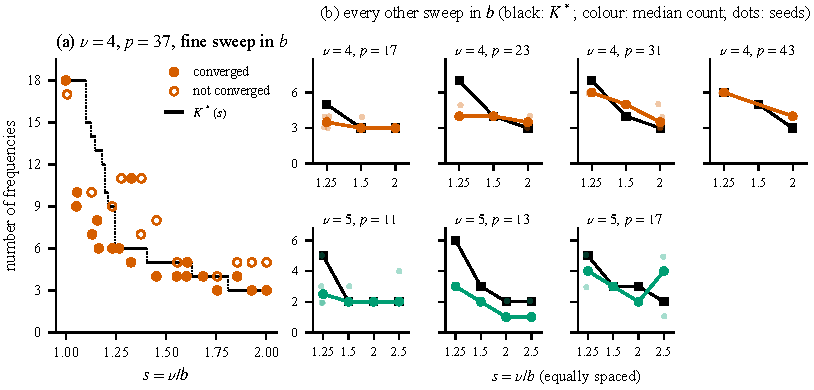
\includegraphics[width=\linewidth]{figures/fig_exponent.pdf}
\caption{\textbf{The count follows the exponent.} (a) Product networks at $\nu=4$, $p=37$, sweeping $b$ from $4$ to $2$ ($s$ from $1$ to $2$). Black: $\Kstar(s)$, exact, with its twelve plateaus (the two at $\Kstar=6$ differ in their amplitude ratios). Each marker is one run ($19$ converged, $13$ not). (b) Every other sweep in $b$ at fixed $(\nu,p)$ with at least two converged cells ($\nu=4$, $p=59$, where $8$ of $12$ runs diverged, has one and is omitted). Black: $\Kstar$; colour: median count over converged seeds; dots: individual seeds. The $s$ values are drawn equally spaced.}
\label{fig:exponent}
\end{figure}

Sweeping the norm exponent at fixed degree and prime (Figure~\ref{fig:exponent}a), the trained count falls with $\Kstar$, from every frequency at $b=\nu$ to three at $b=2$, although it does not resolve the finer plateaus of $\Kstar$. The same holds in every other sweep in $b$ (Figure~\ref{fig:exponent}b and, at $\nu=3$, Figure~\ref{fig:prime}). Across all pairs of settings that share $\nu$ and $p$ but differ in $b$, the trained count moves in the same direction as $\Kstar$ in $30$ of $36$ (Appendix~\ref{app:exp}).

At the dense end, $b=\nu$ ($s=1$, the left end of Figure~\ref{fig:exponent}a), every converged network at $\nu=3$ and $\nu=4$ uses every frequency, most with near-equal amplitudes, as Corollary~\ref{cor:dense} predicts; density alone is not diagnostic, since the network at initialization is already dense, but flatness is. At $\nu=5$ the picture is mixed.

\subsection{Moving the degree and the norm separately}

Theorem~\ref{thm:cyclic} says that the optimal spectral allocation depends on $\nu$ and $b$ only through $s$. At equal $s$, trained networks of different degree use the same number of frequencies to within one in $12$ of $17$ comparisons: gradient descent falls further below $\Kstar$, and further from the optimum, as the degree grows (Appendix~\ref{app:exp}).

\begin{figure}[h!]
\centering
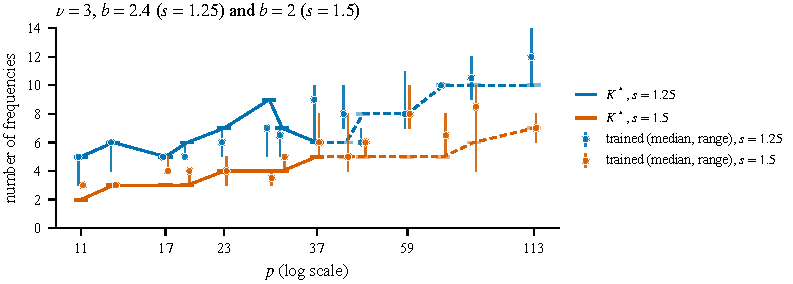
\includegraphics[width=\linewidth]{figures/fig_prime.pdf}
\caption{\textbf{The count across primes}, product networks at $\nu=3$. Lines: $\Kstar$ (solid where exact, $p\le37$; dashed where best found, Appendix~\ref{app:exp}). Markers: median over converged seeds, with the range. $\Kstar$ is not monotone in $p$ (at $s=1.25$ it is $9,7,6$ at $p=29,31,37$); the trained counts do not follow these steps.}
\label{fig:prime}
\end{figure}

Across primes (Figure~\ref{fig:prime}), the count stays within one of $\Kstar$ in most $(p,s)$ cells ($20$ of $28$, against $16$ for the best constant), but it does not follow the non-monotone steps of $\Kstar$.

\FloatBarrier

\section{Discussion}\label{sec:discussion}
% DRAFT for the author to rewrite. Every statement points to where it is shown in the paper.

For modular addition, the number of features a maximum-margin network uses is set by the exponent $s=\nu/b$: every frequency at $b=\nu$, and $\Theta(\log p)$ frequencies for every $b<\nu$ (Theorems~\ref{thm:cyclic} and~\ref{thm:count}). The same programme recovers the dense maxima of \citet{morwani2024feature} and \citet{li2025nsum} at $b=\nu$, and in trained networks the count moves with $s$ in the direction the programme predicts (Section~\ref{sec:experiments}).

\paragraph{Limitations.} The exact optimum of Theorem~\ref{thm:cyclic} is proved for interference-free networks. For all networks we prove only the universal bound and the order of the optimum (Theorems~\ref{thm:universal} and~\ref{thm:scaling}); whether interference can raise the margin for $2\le b<\nu$ is open (Appendix~\ref{app:conjecture}). The results concern maximum-margin solutions, which regularized cross-entropy reaches only at its global minimizers as $\lambda\to0$ \citep{wei2019regularization}; gradient descent need not find them. Accordingly, trained networks carry some interference and are not maximizers of the programme, so our experiments test trends in the count rather than exact values: they do not resolve the finer plateaus of $\Kstar$ or its non-monotone steps in $p$, and they fall further below $\Kstar$ as the degree grows. For power networks we prove the same upper bounds (with constant $n!B_p$), but they are known to be attained only at $b=\nu$ \citep{li2025nsum}, so the exact optimum and the logarithmic laws are proved for product networks only (Appendix~\ref{app:conjecture}). Finally, the theory covers sums of such neurons over the cyclic group $\sZ_p$; networks with a shared linear layer in front of the neurons are priced by a nuclear norm and fall outside it (Appendix~\ref{app:models}), and other groups are not treated here.


\clearpage
% ---------------------------------------------------------------------------------------------
% AI use statement (required, outside the page limit, max 1 page). Structure follows the template
% in iclr2027_conference.tex l.397-412. Categories are quoted from the ICLR 2027 AI Policy for Authors.
% The same disclosure must also be entered on the OpenReview submission form.
%
% REQUIRED-disclosure categories -- tick each one as USED, NOT USED, or N/A:
%   [ ] generate synthetic data sets                          -> likely N/A (the data is the full table D_p)
%   [ ] help develop theoretical models / conceptual frameworks
%   [ ] formulate mathematical claims
%   [ ] provide critical ingredients for proving mathematical claims
%   [ ] assist in the writing of proofs
%   [ ] propose or refine hypotheses
%   [ ] design or provide feedback on research methodology or experiments
%   [ ] implement methods                                      -> USED (training and analysis code in the supplement)
%   [ ] assist with translation                                -> likely N/A
%   [ ] clean and reformat dataset                             -> likely N/A
%   [ ] support qualitative and thematic data analysis         -> likely N/A
%   [ ] interpret results
% RECOMMENDED-disclosure categories (disclose whichever apply):
%   create/modify figures; suggest experimental parameters; create/edit code; create artifacts;
%   draft parts of the paper; summarize/analyse literature; identify gaps; brainstorming;
%   searching for information; edit for readability; identify relevant literature; format references;
%   suggest a paper structure; propose a title or keywords.
% Anything in \aifill{...} is a prompt for the author; delete the macro once the text is final.
% ---------------------------------------------------------------------------------------------
\providecommand{\aifill}[1]{\textbf{[#1]}}

\section*{AI use statement}

In this work, we used generative AI tools to design, and give feedback on, the research methodology and experiments, implement methods, provide critical ingredients for proving mathematical claims, interpret results and assist in the writing of proofs.
We have not used generative AI tools to help develop theoretical models or conceptual frameworks, formulate mathematical claims and propose or refine hypotheses,
and generating synthetic data sets, assisting with translation, cleaning and reformatting datasets, and qualitative and thematic data analysis are not applicable to this work.
Additionally, we used generative AI tools to create and edit software code, create the figures, suggest experimental parameters, build the supplementary material, draft parts of the paper (Section~\ref{sec:experiments} and Appendix~\ref{app:exp}), edit the paper for readability, search for, identify, summarize and analyse existing literature, format references, brainstorm, identify gaps and suggest a structure for the paper. 
We have reviewed all AI-assisted work. All proofs that were AI-assisted were verified by the authors and Lean 4, a literature survey was undertaken to prevent plagiarism and LLM-generated code was hand-reviewed.
We take responsibility for the final content of this work, including text, claims or artifacts produced with the aid of generative AI.


\section*{Reproducibility statement}
All theorems are stated with their hypotheses in Sections~\ref{sec:approach} and~\ref{sec:cyclic} and proved in full in Appendices~\ref{app:approach} and~\ref{app:cyclic}; Appendix~\ref{app:models} checks the assumptions for concrete networks. The data are the full table $D_p$ of Section~\ref{sec:prelim}, with no split or preprocessing. Appendix~\ref{app:exp} gives the training recipe, the convergence criterion and the definition of the feature count. The anonymized supplementary material contains the code, with scripts that regenerate the predictions, runs and analyses; the trained weights and full configuration of every run; a list of every launched run with its status; the preregistrations, with the post-hoc analyses reported separately; an audit of the training code against the stated recipe; and a file, \texttt{results.json}, that links every number in the paper, including the numerical checks of Section~\ref{sec:cyclic}, to the script that computes it.

\clearpage
\bibliography{refs}
\bibliographystyle{iclr2027_conference}

\newpage
\appendix
\section*{Appendix}
\textbf{Appendix organization.} Appendix~\ref{app:approach} proves the results of Section~\ref{sec:approach}, including the price of a feature (Lemma~\ref{lem:price}). Appendix~\ref{app:cyclic} proves the results of Section~\ref{sec:cyclic}: the cost of a feature (Lemma~\ref{lem:cost}), Theorem~\ref{thm:cyclic}, the $\nu$-block (Proposition~\ref{prop:block}), two facts about the programme (Lemmas~\ref{lem:vertex} and~\ref{lem:ablation}) and logarithmic scaling (Theorems~\ref{thm:scaling} and~\ref{thm:count}, Corollary~\ref{cor:few}). Appendix~\ref{app:models} computes the single-neuron budget and checks the sign rule for the product and power networks. Appendix~\ref{app:conjecture} states the conjecture that the interference-free value is the global maximum, and what is known about it.

Throughout, for $v:\sZ_p\to\R$ we use $\hat v(j)=\sum_av(a)\rho^{-ja}$, so that $v(a)=p^{-1}\sum_j\hat v(j)\rho^{ja}$, $\sum_{j\in\sZ_p}|\hat v(j)|^2=p\|v\|_2^2$ (Parseval), $\hat v(-j)=\overline{\hat v(j)}$, and hence $\sum_{j\in\Fp}|\hat v(j)|^2\le\frac p2\|v\|_2^2$.

\section{Proofs for Section~\ref{sec:approach}}\label{app:approach}

\subsection{The spectrum of the averaged logit}\label{app:spectrum}

Write the logit table through its multidimensional Fourier transform,
$f(\theta,x)[c]=p^{-(n+1)}\sum_{k_1,\dots,k_n,l}\hat f_\theta(k_1,\dots,k_n;l)\,\rho^{k_1a_1+\dots+k_na_n+lc}$. Substituting $c=y(x)-\delta=a_1+\dots+a_n-\delta$ and averaging over $x$,
\[
\eta_\theta(\delta)=p^{-(n+1)}\sum_{k,l}\hat f_\theta(k;l)\,\rho^{-l\delta}\prod_{t=1}^n\E_{a_t}\big[\rho^{(k_t+l)a_t}\big].
\]
Each average is $1$ if $k_t=-l$ and $0$ otherwise, so only the modes $(j,\dots,j;-j)$ survive (with $j=-l$):
\[
\eta_\theta(\delta)=p^{-(n+1)}\sum_{j\in\sZ_p}G_j\,\rho^{j\delta},\qquad G_j:=\hat f_\theta(j,\dots,j;-j).
\]
Since the table is real, $G_{-j}=\overline{G_j}$, and pairing $j$ with $-j$ gives \eqref{eq:spectrum} with $\bar\eta_\theta=p^{-(n+1)}G_0$ and $\beta_j=2p^{-(n+1)}G_j$. The averaged form used in Lemma~\ref{lem:phase} is
\[
\eta_\theta(0)-\tfrac12\big(\eta_\theta(\delta)+\eta_\theta(-\delta)\big)=\sum_{j\in\Fp}\mathrm{Re}(\beta_j)\big(1-\cos(2\pi j\delta/p)\big)=\sum_{j\in\Fp}\mathrm{Re}(\beta_j)\,\cov{j}{\delta},
\]
because $\mathrm{Re}(\beta\rho^{j\delta})+\mathrm{Re}(\beta\rho^{-j\delta})=2\,\mathrm{Re}(\beta)\cos(2\pi j\delta/p)$. The same computation for one neuron defines $\beta_{ij}$. For a product neuron $\hat f$ factorizes, so $G_{ij}=\hat u_{i1}(j)\cdots\hat u_{in}(j)\,\hat w_i(-j)$, and $p^{-(n+1)}=p^{-\nu}$.

\subsection{Proof of Lemma~\ref{lem:phase}}\label{app:phase}

Fix $\delta\neq0$. Then $-\delta\neq0$ as well, so Lemma~\ref{lem:avg} applies at both offsets:
\[
h(\theta)\le\eta_\theta(0)-\eta_\theta(\delta),\qquad h(\theta)\le\eta_\theta(0)-\eta_\theta(-\delta).
\]
Averaging the two and using the identity of Appendix~\ref{app:spectrum},
\[
h(\theta)\le\eta_\theta(0)-\tfrac12\big(\eta_\theta(\delta)+\eta_\theta(-\delta)\big)=\sum_{j\in\Fp}\mathrm{Re}(\beta_j)\,\cov{j}{\delta}.
\]
This is the first inequality. For the second, $\cov{j}{\delta}=1-\cos(2\pi j\delta/p)\ge0$ and $\mathrm{Re}(\beta_j)\le|\beta_j|=A_j$, so each term is at most $A_j\cov{j}{\delta}$. Equality in the second step requires $\mathrm{Re}(\beta_j)=A_j$, i.e.\ $\beta_j$ real and non-negative, at every $j$ with $\cov{j}{\delta}>0$.
\qed

\subsection{The price of a feature}\label{app:price}

This makes precise the price used in Section~\ref{sec:programme}; Appendix~\ref{app:models} proves the general single-neuron budget, of which this is the single-frequency case.

\begin{lemma}[price of an amplitude]\label{lem:price}
Let $\omega=(u_1,\dots,u_n,w)$ be a product neuron whose $\nu=n+1$ weight vectors are real and supported on the frequencies $\pm j$ for one $j\in\Fp$, and let $A=|\beta_j(\omega)|$. Then for every $b>0$,
\[
\|\omega\|_2^b\ \ge\ \big(A/B_p\big)^{b/\nu},\qquad B_p=2(2p\nu)^{-\nu/2},
\]
with equality if and only if the $\nu$ weight vectors have equal norm. So the least $L_{2,b}$ penalty that buys amplitude $A$ is $B_p^{-1/s}A^{1/s}$ with $s=\nu/b$.
\end{lemma}
\begin{proof}
Write $v_1,\dots,v_\nu$ for $u_1,\dots,u_n,w$ and $x_t=\|v_t\|_2$. A real vector supported on $\pm j$ has $|\hat v(-j)|=|\hat v(j)|$ and no other Fourier content, so Parseval gives $x_t^2=\frac2p|\hat v_t(j)|^2$. By Appendix~\ref{app:spectrum}, $A=2p^{-\nu}\prod_t|\hat v_t(j)|=2p^{-\nu}(p/2)^{\nu/2}\prod_tx_t$. By AM--GM, $\|\omega\|_2^2=\sum_tx_t^2\ge\nu\big(\prod_tx_t\big)^{2/\nu}$, with equality if and only if all $x_t$ are equal. Hence
\[
\|\omega\|_2^2\ \ge\ \nu\Big(\frac{A}{2p^{-\nu}(p/2)^{\nu/2}}\Big)^{2/\nu}=\Big(\frac{A}{2p^{-\nu}(p/(2\nu))^{\nu/2}}\Big)^{2/\nu}=\big(A/B_p\big)^{2/\nu},
\]
and raising to the power $b/2$ gives the claim, since $t\mapsto t^{b/2}$ is increasing.
\end{proof}

For a power neuron with the same weight vectors, only the multilinear term of $\big(\sum_tu_t(a_t)\big)^n$ reaches the mode $(j,\dots,j;-j)$, so $A=n!\cdot2p^{-\nu}\prod_t|\hat v_t(j)|$ (Appendix~\ref{app:models}); the same proof gives $\|\omega\|_2^b\ge\big(A/(n!\,B_p)\big)^{b/\nu}$.

The inner norm of $L_{2,b}$ must be $\ell_2$ for this argument: Parseval converts it to Fourier magnitudes, and AM--GM then acts on the squared factor norms. The outer exponent $b$ only raises each neuron's cost to the power $b/2$, which turns the product of $\nu$ factors into the exponent $b/\nu=1/s$.

\subsection{The dense endpoint \texorpdfstring{$b=\nu$}{b = nu}}\label{app:dense}

\begin{corollary}[$b=\nu$: every frequency is used]\label{cor:dense}
$\Gamma_1(p)=p/(p-1)$, with unique maximizer $y_j=2/(p-1)$ for all $j$, so at $b=\nu$ any network attaining Theorem~\ref{thm:universal} has equal amplitude on every frequency. For the quadratic network of \citet{morwani2024feature} the bound is $2B_p\frac p{p-1}=\sqrt{2/27}\,/\,(p^{1/2}(p-1))$, exactly their maximum $L_{2,3}$-margin \citep[Thm.~7; width $m\ge4(p-1)$]{morwani2024feature}.
\end{corollary}
For the $n$-operand power network, $n!\,B_p\,p/(p-1)$ is the maximum $L_{2,n+1}$-margin of \citet[Thm.~4.1]{li2025nsum}, and equal amplitude on every frequency is already implicit in \citet[App.~F.3]{morwani2024feature}. The value $\Gamma_1(p)=p/(p-1)$ and its flat maximizer are the regular-simplex bound for cyclic codes \citep{rankin1955closest,slepian1968group}.

\emph{Proof of Corollary~\ref{cor:dense}.}

For feasible $y$ (at $s=1$, $\sum_jy_j\le1$),
\[
\min_{\delta\neq0}\sum_jy_j\cov{j}{\delta}\le\frac1{p-1}\sum_{\delta\neq0}\sum_jy_j\cov{j}{\delta}=\frac p{p-1}\sum_jy_j\le\frac p{p-1},
\]
using $\sum_{\delta\neq0}\cov{j}{\delta}=p$. The flat choice $y_j=2/(p-1)$ attains this, as we now show together with uniqueness (the averaging step is the regular-simplex bound of \citealp{rankin1955closest}; cf.\ \citealp[\S3.5--3.6]{fiedler1973algebraic}; the inversion step parallels \citealp[App.~F.3]{morwani2024feature} and \citealp[Lemma~F.2]{li2025nsum}). Equality forces $\sum_jy_j=1$ and the coverage $\sum_jy_j\cov{j}{\delta}$ to be constant in $\delta\neq0$, i.e.\ $\zeta(\delta):=\sum_{j\in\Fp}y_j\cos(2\pi j\delta/p)$ equals a constant $c_0$ for $\delta\neq0$, with $\zeta(0)=1$. So $\zeta=c_0+(1-c_0)[\delta=0]$. Its normalized Fourier coefficients $\frac1p\sum_\delta\zeta(\delta)\rho^{-k\delta}$ are $c_0+(1-c_0)/p$ at $k=0$ and $(1-c_0)/p$ at $k\neq0$. From the cosine form they are $0$ at $k=0$ and $y_j/2$ at $k=\pm j$. Hence $c_0=-1/(p-1)$ and $y_j=2(1-c_0)/p=2/(p-1)$ for every $j$.

For the product network, attainment is Proposition~\ref{prop:block} at $b=\nu$ with $y^*$ flat. The equality conditions are those of Proposition~\ref{prop:coverage} (flat amplitudes) and of the triangle inequality (at each $j$, all non-zero $\beta_{ij}$ have the same phase). For the quadratic network of \citet{morwani2024feature}, $C_3=2B_p$ (Appendix~\ref{app:models}), and $2B_p\cdot\frac p{p-1}=4(6p)^{-3/2}\frac p{p-1}=\frac{2}{3\sqrt6}\cdot\frac1{p^{1/2}(p-1)}=\sqrt{\frac2{27}}\cdot\frac1{p^{1/2}(p-1)}$.
\qed

\section{Proofs for Section~\ref{sec:cyclic}}\label{app:cyclic}

\subsection{Proof of Lemma~\ref{lem:cost}}\label{app:cost}

\begin{lemma}[chain lemma]\label{lem:chain}
$\|m_l\|_2^2=\nu$, and $H:=\sum_l\beta_lm_lm_l^*$ is upper triangular with every diagonal entry equal to $\beta$.
\end{lemma}
\begin{proof}
Index the chain coordinates by $0,\dots,n$. Every entry of $m_l$ has modulus $1$, so $\|m_l\|_2^2=\nu$ and the diagonal of $H$ is $\sum_l\beta_l=\beta$. For $t>t'$, the $(t,t')$ entry of $m_lm_l^*$ is $\prod_{u=t'+1}^{t}\xi_{lu}$. Its sum against $\beta_l$ vanishes by \eqref{eq:JF}, applied to the non-empty interval $T=\{t'+1,\dots,t\}$.
\end{proof}
The entries above the diagonal need not vanish: $H$ is triangular, not necessarily Hermitian. Triangularity is all the proof needs.

\begin{proof}[Proof of Lemma~\ref{lem:cost}]
If $\beta=0$, the inequality is immediate, with equality exactly when every $\beta_l=0$. Otherwise divide the coefficients by $\beta$; \eqref{eq:JF} is preserved with total $1$. We prove the normalized claim and restore the factor $|\beta|^r$ at the end. For $r=1$, the claim is simply $\sum_l|\beta_l|\ge|\sum_l\beta_l|=1$. Henceforth let $0<r<1$.

\emph{Step 1: compare determinants.} Put $u_l=m_l/\sqrt\nu$, $d_l=\nu\beta_l$ and $x_l=|d_l|$, so that the $u_l$ are unit vectors and $H=\sum_ld_lu_lu_l^*$. Let $U=[u_1\cdots u_N]$ and $\Delta=\mathrm{diag}(d_1,\dots,d_N)$. Sylvester's determinant theorem $\det(I+AB)=\det(I+BA)$ \citep[Ch.~1]{horn2012matrix} and expansion by principal minors give
\begin{equation}
\det(I_\nu+tH)=\det(I_N+t\Delta U^*U)
=\sum_{L\subseteq[N]}t^{|L|}\Big(\prod_{l\in L}d_l\Big)G_L,
\qquad G_L:=\det\mathrm{Gram}(u_l:l\in L).
\label{eq:cost-minors}
\end{equation}
Gram positivity and Hadamard's inequality \citep[Ch.~7]{horn2012matrix} give $0\le G_L\le1$, with $G_L=1$ exactly when the vectors in $L$ are orthonormal. By Lemma~\ref{lem:chain}, $\det(I+tH)=(1+t)^\nu$. Taking absolute values in \eqref{eq:cost-minors} therefore yields, for $t\ge0$,
\begin{equation}
(1+t)^\nu\le\sum_{L\subseteq[N]}t^{|L|}\prod_{l\in L}x_l
=\prod_{l=1}^N(1+tx_l).
\label{eq:cost-generating}
\end{equation}
The same comparison coefficient by coefficient gives $e_k(x)\ge\binom\nu k$ for $0\le k\le\nu$, where $e_k$ is the $k$th elementary symmetric polynomial; in particular, at least $\nu$ coefficients are non-zero.

\emph{Step 2: integrate the logarithm.} Define
\[
J_r(x):=\int_0^\infty\log(1+xt)\,t^{-1-r}\,dt,\qquad x\ge0.
\]
For $x>0$ the integrand is $O(t^{-r})$ near zero and $O(t^{-1-r}\log t)$ near infinity, so the integral converges. Substitution gives $J_r(x)=x^rJ_r(1)$, also valid at $x=0$, with $0<J_r(1)<\infty$. Integrating the logarithm of \eqref{eq:cost-generating} against $t^{-1-r}dt$ and cancelling $J_r(1)$ gives
\[
J_r(1)\sum_lx_l^r=\sum_lJ_r(x_l)\ge\nu J_r(1),
\qquad\text{hence}\qquad \sum_lx_l^r\ge\nu.
\]
Restoring the original coefficients, $x_l=\nu|\beta_l|/|\beta|$, proves $\sum_l|\beta_l|^r\ge\nu^{1-r}|\beta|^r$.

\emph{Step 3: characterize equality.} At equality, the continuous non-negative function $\sum_l\log(1+x_lt)-\nu\log(1+t)$ has zero integral against a strictly positive density, so it vanishes for every $t>0$. Thus $\prod_l(1+x_lt)=(1+t)^\nu$ as polynomials. Their roots show that the non-zero $x_l$ are exactly $\nu$ copies of $1$. Let $L_0$ be their support. Comparing the coefficient of $t^\nu$ in \eqref{eq:cost-minors} gives $1=(\prod_{l\in L_0}d_l)G_{L_0}$. Since $|\prod_{l\in L_0}d_l|=1$, we have $G_{L_0}=1$: the corresponding $u_l$ are orthonormal, and the chain vectors $m_l$ are orthogonal. Conversely, exactly $\nu$ non-zero coefficients of modulus $|\beta|/\nu$ satisfying \eqref{eq:JF} give $\sum_l|\beta_l|^r=\nu^{1-r}|\beta|^r$.
\end{proof}

\begin{remark}[orthogonality as roots of unity]
Two chain vectors $m_l,m_{l'}$ are orthogonal if and only if $\sum_{t=0}^n\prod_{u\le t}\xi_{l'u}\overline{\xi_{lu}}=0$. If the ratios $\xi_{l'u}\overline{\xi_{lu}}=\zeta$ agree across operands, this reads $1+\zeta+\dots+\zeta^n=0$: $\zeta$ is a non-trivial $\nu$\textsuperscript{th} root of unity. This is the configuration of Proposition~\ref{prop:block}.
\end{remark}

\begin{remark}[other penalties]
For $0<r<1$, $x\mapsto x^r$ is a positive integral of the functions $x\mapsto\log(1+xt)$. The same proof, together with $\sum_lx_l\ge\nu$, gives $\sum_l\psi(\nu|\beta_l|/|\beta|)\ge\nu\,\psi(1)$ for every $\psi(x)=cx+\int_0^\infty\log(1+xt)\,\mu(dt)$ with $c\ge0$ and $\mu\ge0$, whenever these integrals are finite and $\beta\neq0$. The result is not special to power penalties (the admissible $\psi$ are Thorin--Bernstein functions, \citealp[Ch.~8]{schilling2012bernstein}; for the inequality alone see also \citealp{thompson1976convex}).
\end{remark}

\subsection{Proof of Theorem~\ref{thm:cyclic}}\label{app:thm}

Let $r=b/\nu$, so $1/r=s$.

\emph{Upper bound.} Let $\theta$ be interference-free. At each $j\in\Fp$, the coefficients $(\beta_{ij})_i$ satisfy \eqref{eq:JF} with total $\beta_j$: for $T=\emptyset$ this is $\beta_j=\sum_i\beta_{ij}$, and for $T\neq\emptyset$ it is $0=\beta_{j,T}=\sum_i\beta_{ij}\prod_{t\in T}\xi_{itj}$ by Lemma~\ref{lem:sign}. Lemma~\ref{lem:cost} gives $\sum_i|\beta_{ij}|^r\ge\nu^{1-r}A_j^r$. Summing over $j$ and using the single-neuron budget,
\begin{equation}
\nu^{1-r}\sum_jA_j^r\ \le\ \sum_i\sum_j|\beta_{ij}|^r\ \le\ C_b\sum_i\|\omega_i\|_2^b=C_b\|\theta\|_{2,b}^b .
\label{eq:chain}
\end{equation}
Raising to the power $1/r$, $\|A\|_{1/s}\le\nu^{(r-1)/r}C_b^{1/r}\|\theta\|_{2,b}^{b/r}=\nu^{-(\nu-b)/b}B_p\|\theta\|_{2,b}^{\nu}$, and Proposition~\ref{prop:coverage} gives $h(\theta)\le\nu^{-(\nu-b)/b}B_p\Gamma_s(p)\|\theta\|_{2,b}^\nu$.

\emph{Attainment.} Proposition~\ref{prop:block} gives an interference-free network with $\nu|\spt(y^*)|$ neurons attaining the value; any further neurons are set to zero.

\emph{Structure ($b<\nu$).} Let $\theta$ be interference-free and attain the value. The value is positive, so $h(\theta)>0$ and $A\neq0$. The two inequalities $h(\theta)\le\Gamma_s(p)\|A\|_{1/s}$ and $\|A\|_{1/s}\le\nu^{-(\nu-b)/b}B_p\|\theta\|_{2,b}^\nu$ must both be equalities. For the first, write $y=A/\|A\|_{1/s}$; by Lemma~\ref{lem:phase}, $h(\theta)\le\|A\|_{1/s}\min_{\delta\neq0}\sum_jy_j\cov{j}{\delta}\le\|A\|_{1/s}\Gamma_s(p)$, so equality forces $\min_\delta\sum_jy_j\cov{j}{\delta}=\Gamma_s(p)$: $y$ is a maximizer of \eqref{eq:programme}, which is condition~1 with $c=\|A\|_{1/s}$. For the second, the first inequality of \eqref{eq:chain} is an equality. It is a sum over $j$ of the inequalities $\sum_i|\beta_{ij}|^r\ge\nu^{1-r}A_j^r$, so each of these is an equality. At a frequency with $A_j>0$, the equality case of Lemma~\ref{lem:cost} ($r<1$) is condition~2. At a frequency with $A_j=0$ it forces $\beta_{ij}=0$ for every $i$: no neuron carries an unused frequency.
\qed

\subsection{Proof of Proposition~\ref{prop:block}}\label{app:block}

\emph{Identity.} Write $\vartheta_t=2\pi ja_t/p$ and $\vartheta_c=2\pi jc/p$, and expand each cosine into exponentials. Neuron $l$ contributes
\[
2^{-\nu}\lambda^\nu\sum_{\varepsilon\in\{\pm1\}^n,\ \varepsilon_c=\pm1}\exp\!\big(i(\varepsilon\cdot\vartheta+\varepsilon_c\vartheta_c)\big)\,\exp\!\Big(i\alpha_l\big(\textstyle\sum_t\varepsilon_t+n\varepsilon_c\big)\Big).
\]
With $N_-=|\{t:\varepsilon_t=-1\}|$ we have $\sum_t\varepsilon_t=n-2N_-$, so the $l$-dependent phase is $\exp(2\pi i\,lu/\nu)$ with $u=n-N_-$ if $\varepsilon_c=+1$ and $u=-N_-$ if $\varepsilon_c=-1$. Summing over $l=0,\dots,n$ gives $\nu\,[u\equiv0\bmod\nu]$. As $0\le N_-\le n$, this happens only for $(N_-=n,\varepsilon_c=+1)$ and $(N_-=0,\varepsilon_c=-1)$, i.e.\ for $e^{\mp i(\sum_t\vartheta_t-\vartheta_c)}$, whose sum is $2\cos(\sum_t\vartheta_t-\vartheta_c)$. The block's table is therefore $\nu\lambda^\nu2^{-n}\cos\big(2\pi j(a_1+\dots+a_n-c)/p\big)$. For the cost, $\sum_a\cos^2(2\pi ja/p+\alpha)=p/2$ for $j\not\equiv0$, so each of the $\nu$ weight vectors of neuron $l$ has squared norm $\lambda^2p/2$.

\emph{Attainment.} Let $r=b/\nu$ and $s=1/r$. Scaling $y^*$ up increases the objective, so $\sum_j(y^*_j)^r=1$. With $\nu\lambda_j^\nu2^{-n}=y^*_j$ the network's table is exactly
$f(\theta,x)[c]=\sum_jy^*_j\cos\big(2\pi j(y(x)-c)/p\big)$. It depends only on $y(x)-c$, so it is interference-free, and on every input $f(\theta,x)[y(x)]-f(\theta,x)[y(x)-\delta]=\sum_jy^*_j\cov{j}{\delta}$; hence $h(\theta)=\min_{\delta\neq0}\sum_jy^*_j\cov{j}{\delta}=\Gamma_s(p)$. For any non-negative allocation $y$, the same construction has penalty
\[
P_b:=\|\theta\|_{2,b}^b
=\sum_j\nu(\nu p/2)^{b/2}(2^ny_j/\nu)^r
=\nu^{1-r}B_p^{-r}\sum_jy_j^r.
\]
For $y=y^*$ the last sum is one. Thus $\|\theta\|_{2,b}^\nu=P_b^{1/r}=\nu^{s-1}B_p^{-1}$, and
\[
\frac{h(\theta)}{\|\theta\|_{2,b}^\nu}
=\nu^{1-s}B_p\Gamma_s(p),
\]
as claimed. More generally, any $y$ with $\sum_jy_j^r=1$ gives normalized margin $\nu^{1-s}B_p\min_{\delta\neq0}\sum_jy_j\cov{j}{\delta}$.
\qed

\subsection{Two facts about the programme}\label{app:shape}

Throughout, $s>1$, $r=1/s<1$, and $\phi(v):=\sum_jv_j^r$. Rescaling a feasible $y$ so that its worst coverage is one puts it in the polyhedron
\[
\curlyp_p:=\Big\{v\in\R_{\ge0}^{\Fp}:\ \textstyle\sum_{j\in\Fp}v_j\,\cov{j}{\delta}\ge1\ \text{ for all }\delta\neq0\Big\}.
\]
If $y$ is feasible for \eqref{eq:programme} with worst coverage $m>0$, then $v=y/m\in\curlyp_p$ and $\phi(v)=m^{-r}\sum_jy_j^r\le m^{-r}$. Conversely, for $v\in\curlyp_p$ the vector $y=v/\phi(v)^s$ is feasible with worst coverage at least $\phi(v)^{-s}$. Hence $\Gamma_s(p)=(\min_{\curlyp_p}\phi)^{-s}$. A maximizer has $\sum_jy_j^r=1$, since scaling up raises the objective. So $y$ is a maximizer if and only if $y=\Gamma_s(p)\,v$ with $v$ a minimizer of $\phi$ over $\curlyp_p$.

\begin{lemma}[maximizers are vertices]\label{lem:vertex}
Let $s>1$. Every maximizer of \eqref{eq:programme} is $y=\Gamma_s(p)\,v$ for a vertex $v$ of $\curlyp_p$ that minimizes $\sum_jv_j^{1/s}$.
\end{lemma}
\begin{proof}
This is the classical fact that concave functions attain their minima over a polyhedron at vertices \citep[\S32]{hirsch1961extreme,rockafellar1970convex}. The polyhedron $\curlyp_p$ is nonempty and closed. Since $v_j\le\phi(v)^{1/r}$ for every $j$, the sublevel sets of $\phi$ in $\curlyp_p$ are compact, so a minimum exists. If a minimizer $v$ were not a vertex, it would be the midpoint of distinct $v',v''\in\curlyp_p$. Strict concavity of $t\mapsto t^r$ on $[0,\infty)$ would give $\phi(v)>\frac12(\phi(v')+\phi(v''))\ge\min\phi$, a contradiction.
\end{proof}
The vertex set is finite, so $\Kstar$ can be computed exactly by enumerating the supports of vertices (Table~\ref{tab:kstar}); in general this minimization is NP-hard \citep{ge2011note}.

\begin{lemma}[removing a feature]\label{lem:ablation}
Let $s>1$. Let $y$ be feasible for \eqref{eq:programme} with $\sum_jy_j^{1/s}=1$ and worst coverage $m\ge(1-\varepsilon)\,\Gamma_s(p)$, where $\varepsilon\in[0,1)$. For $j\in\spt(y)$, let $w_j:=y_j^{1/s}$ be the share of the budget spent on $j$, and let $m_{-j}$ be the worst coverage after setting $y_j=0$. Then
\[
m-2y_j\ \le\ m_{-j}\ \le\ \frac{(1-w_j)^s}{1-\varepsilon}\,m .
\]
In particular, removing feature $j$ from a maximizer costs at least the fraction $1-(1-w_j)^s\in[w_j,s\,w_j]$ of the worst coverage.
\end{lemma}
\begin{proof}
Removing frequency $j$ decreases every offset's coverage by at most $2y_j$, proving the lower bound. For the upper bound, if $w_j=1$ then $m_{-j}=0$. Otherwise, set $y_j=0$ and multiply the remaining amplitudes by $(1-w_j)^{-s}$. The resulting allocation has budget one, so its worst coverage obeys $(1-w_j)^{-s}m_{-j}\le\Gamma_s(p)\le m/(1-\varepsilon)$. Finally, $(1-w)^s\le1-w$ and Bernoulli's inequality $(1-w)^s\ge1-sw$ give $w\le1-(1-w)^s\le sw$.
\end{proof}
In the network of Proposition~\ref{prop:block}, deleting the $\nu$ neurons of frequency $j$ removes exactly $y_j\cos(2\pi j(a_1+\dots+a_n-c)/p)$ from the table, so these bounds apply to its margin directly. Lemma~\ref{lem:ablation} is used in the proof of Theorem~\ref{thm:count}.

\subsection{Proof of Theorems~\ref{thm:scaling} and~\ref{thm:count} and Corollary~\ref{cor:few}}\label{app:scaling}

Write $F_y(\delta):=\sum_{j\in\Fp}y_j\cov{j}{\delta}$ and $m(y):=\min_{\delta\neq0}F_y(\delta)$. Let $r=1/s$ and $a_s=3+s/2$; logarithms are natural. The constants below are chosen for simplicity, not sharpness.

\emph{Lower bound.} Let $L=\lceil8\ln p\rceil$ and draw $J_1,\dots,J_L$ independently and uniformly from $\Fp$. For fixed $\delta\neq0$,
\[
\E\cos(2\pi J_1\delta/p)=\frac2{p-1}\sum_{j\in\Fp}\cos(2\pi j\delta/p)=-\frac1{p-1}.
\]
By Hoeffding's inequality for variables in $[-1,1]$ \citep[Thm.~2]{hoeffding1963probability}, $\Pr\big[\frac1L\sum_\ell\cos(2\pi J_\ell\delta/p)>\frac12\big]\le e^{-L/8}\le\frac1p$. A union bound over the $p-1$ offsets leaves positive probability that $\sum_\ell\cov{J_\ell}{\delta}\ge L/2$ for every $\delta\neq0$; fix such a draw.
Let $n_j$ be the multiplicity of $j$ in the draw and set $y_j=n_jL^{-s}$. Then
\[
q:=\sum_jy_j^r=L^{-1}\sum_jn_j^r\le1,
\qquad
F_y(\delta)=L^{-s}\sum_\ell\cov{J_\ell}{\delta}\ge\tfrac12L^{1-s}.
\]
Here $q>0$. Replacing $y$ by $y/q^s$ makes the budget exactly one, preserves its support, and can only increase coverage. Thus the lower bound is achieved by a feasible allocation using at most $L$ frequencies. Since $L\le9\ln p$ for $p\ge3$, also $\Gamma_s(p)\ge\frac12(9\ln p)^{1-s}$. This is the cyclic case of the random Cayley graph argument of \citet[Sec.~3, Thm.~2]{alon1994random}; cf.\ \citet[Thm.~4.7]{mccracken2025}.

\emph{A positive-Fourier inequality.} If every non-zero offset had large coverage, the average of $e^{-tF_y(\delta)}$ would be small. Positivity of Fourier coefficients forces the same average to remain large under a bounded amplitude budget; comparing the two estimates will bound the margin.

Let $I_0(z)=\frac1\pi\int_0^\pi e^{z\cos\vartheta}d\vartheta$ and $\psi(z)=z-\ln I_0(z)$. For $z\ge0$, the identity
\[
e^{z\cos\vartheta}=\exp\big((z/2)e^{i\vartheta}\big)\exp\big((z/2)e^{-i\vartheta}\big)
\]
and the absolutely convergent exponential series show that all Fourier coefficients are non-negative, with constant coefficient $I_0(z)$ \citep[Eqs.~10.32.1, 10.35.2]{dlmf}. Expand each factor of $e^{-tF_y(\delta)}=\prod_je^{-ty_j}e^{ty_j\cos(2\pi j\delta/p)}$ and average over $\delta\in\sZ_p$. The average keeps the products whose frequencies sum to $0\bmod p$. All are non-negative, and they include the product of the constant terms. Hence, for $t\ge0$,
\begin{equation}
\frac1p\sum_{\delta\in\sZ_p}e^{-tF_y(\delta)}\ \ge\ \prod_je^{-ty_j}I_0(ty_j)=\exp\Big(-\sum_j\psi(ty_j)\Big).
\label{eq:posfourier}
\end{equation}
No independence of the phases $j\delta$ is used: resonances only add non-negative terms (cf.\ the closed-walk comparison of \citealp{cioaba2006closed}).

\emph{A scalar bound.} We claim $0\le\psi(z)\le a_s\ln(1+z^r)$ for $z\ge0$.
\begin{itemize}
\item Non-negativity: $I_0(z)\le e^z$.
\item For $z\le1$: $I_0\ge1$ gives $\psi(z)\le z$. Also $\ln(1+z^r)\ge z^r/2\ge z/2$ and $a_s\ge2$.
\item For $z\ge1$: integrating only over $\vartheta\le z^{-1/2}$ and using $\cos\vartheta\ge1-\vartheta^2/2$ gives $I_0(z)\ge e^{z-1/2}/(\pi\sqrt z)$, so $\psi(z)\le\ln\pi+\frac12+\frac12\ln z$. Meanwhile $3\ln(1+z^r)\ge3\ln2>\ln\pi+\frac12$, and $\frac s2\ln(1+z^r)\ge\frac12\ln z$.
\end{itemize}

If $K\ge1$ and $y$ has at most $K$ non-zero entries and $\sum_jy_j^r\le1$, concavity of the logarithm then gives
\begin{equation}
\sum_j\psi(ty_j)\ \le\ a_s\sum_j\ln(1+t^ry_j^r)\ \le\ a_sK\ln(1+t^r/K)\ \le\ a_st^r .
\label{eq:psisum}
\end{equation}

\emph{Upper bounds.} Since $F_y(0)=0$ and $F_y(\delta)\ge m(y)$ otherwise,
\begin{equation}
\frac1p\sum_\delta e^{-tF_y(\delta)}\le\frac1p+e^{-tm(y)}.
\label{eq:twoterms}
\end{equation}
\begin{itemize}
\item Take $t=(\ln p/(2a_s))^s$. By \eqref{eq:posfourier}--\eqref{eq:twoterms}, $e^{-tm}\ge p^{-1/2}-p^{-1}\ge p^{-1/2}/3$, so $m(y)\le(\frac12\ln p+\ln3)/t\le\frac32(2a_s)^s(\ln p)^{1-s}$ for every feasible $y$.
\item Keeping $K$ in \eqref{eq:psisum} and taking $t^r=K(p^{1/(2a_sK)}-1)$ instead gives, for every feasible $y$ with at most $K$ non-zero entries,
\end{itemize}
\begin{equation}
m(y)\ \le\ \tfrac32(\ln p)^{1-s}\Big(\frac{x}{e^{x/(2a_s)}-1}\Big)^s,\qquad x=\ln p/K.
\label{eq:Kbound}
\end{equation}

\emph{Number of frequencies (Theorem~\ref{thm:count}).}
\begin{itemize}
\item Lower bound. A maximizer has $m=\Gamma_s(p)\ge\tfrac12\,9^{1-s}(\ln p)^{1-s}$. With \eqref{eq:Kbound} and $e^z-1\ge z^2/2$ this gives $\tfrac12\,9^{1-s}\le\frac32(8a_s^2/x)^s$, i.e.\ $K=\ln p/x\ge\ln p/\big(8a_s^2(3\cdot9^{s-1})^{1/s}\big)$.
\item Upper bound. Lemma~\ref{lem:ablation} with $\varepsilon=0$ gives $m-2y_j\le(1-w_j)^sm$. So $2y_j\ge m(1-(1-w_j)^s)\ge m\,w_j=m\,y_j^r$, i.e.\ $w_j\ge(m/2)^{1/(s-1)}$. As $\sum_jw_j=1$, $K\le(2/m)^{1/(s-1)}\le4^{1/(s-1)}L\le9\cdot4^{1/(s-1)}\ln p$, and every share is at least $4^{-1/(s-1)}/L\ge4^{-1/(s-1)}/(9\ln p)$. Keeping $L=\lceil8\ln p\rceil$ gives the dense-regime bound in the main text whenever $|\Fp|>L$.
\end{itemize}

\emph{Networks.} Write $\gamma^*_{b,m}(p)$ for the maximum margin at width $m$. The universal bound gives $\gamma^*_{b,m}(p)\le B_p\Gamma_s(p)$ for every $m$. The normalized random allocation above uses at most $L$ frequencies, so the block construction gives, for every $m\ge\nu L$,
\[
\tfrac12\nu^{1-s}B_pL^{1-s}\le\gamma^*_{b,m}(p)\le B_p\Gamma_s(p).
\]
Together with the programme upper bound and $B_p=2(2p\nu)^{-\nu/2}$, this proves the stated order uniformly over these widths. If $m$ is also large enough to realize a programme maximizer, Theorem~\ref{thm:cyclic} gives the stronger lower bound $\nu^{1-s}B_p\Gamma_s(p)$.

\emph{Corollary~\ref{cor:few}.} If $A=0$, Lemma~\ref{lem:phase} gives $h(\theta)\le0$, so the claim is immediate. Otherwise $y=A/\|A\|_{1/s}$ has budget one and at most $K$ non-zero entries. Lemma~\ref{lem:phase}, the budget estimate in Theorem~\ref{thm:universal}, and \eqref{eq:Kbound} give
\[
h(\theta)\le\|A\|_{1/s}m(y),\qquad
\|A\|_{1/s}\le C_b^{\nu/b}\|\theta\|_{2,b}^\nu,
\]
which prove the displayed bound. For product networks, $C_b^{\nu/b}=B_p$. At any comparison width $m\ge\nu L$, the lower bound just proved shows that the ratio to $\gamma^*_{b,m}(p)$ is at most
\[
3(9\nu)^{s-1}\Big(\frac{x}{e^{x/(2a_s)}-1}\Big)^s.
\]
This tends to zero as $x=\ln p/K\to\infty$. \qed

\subsection{Further remarks on Section~\ref{sec:cyclic}}\label{app:remarks}

\paragraph{Equal shares.} Restricting \eqref{eq:programme} to equal shares on a set of $K$ frequencies, with $M_K(p):=\max_{|S|=K}\min_{\delta\neq0}\sum_{j\in S}\cov{j}{\delta}$, gives $\Gamma_s(p)\ge\max_KK^{-s}M_K(p)$, a cheap approximation. Since the worst offset is no better than the average, $M_K\le pK/(p-1)$ (cf.\ \citealp[Thm.~2]{slepian1968group}), so $K^{-s}M_K\le\frac p{p-1}K^{1-s}$ decays in $K$ for $s>1$. In Table~\ref{tab:kstar} the equal-share argmax agrees with $\Kstar$ except at $(p,\nu)=(59,3)$, where it gives $6$, and $(113,3)$, where it gives $5$; where adjacent equal-share values are within a few percent, the honest statement is a band of width one.

\paragraph{Shares in the block.} Optimal shares are not equal (at $p=59$, $s=3/2$ they range over $0.15$--$0.25$), and a $\nu$-block with equal amplitudes on the optimal support does not attain Theorem~\ref{thm:cyclic}.

\paragraph{Weaker cancellation suffices.} The inequality of Lemma~\ref{lem:cost} uses only the $\binom\nu2$ interval patterns $T=\{t'+1,\dots,t\}$ of \eqref{eq:JF}. The structure statement of Theorem~\ref{thm:cyclic} still needs the full condition: under the interval patterns alone, the equality set contains configurations that are not interference-free (at $\nu=4$, the pattern $T=\{1,3\}$ can be non-zero at equality).

\paragraph{Other networks.} The upper bound of Theorem~\ref{thm:cyclic} uses only the single-neuron budget and the sign rule. For the power network it holds with $B_p$ replaced by $n!\,B_p$; the product-network attainment construction does not establish sharpness for the power network (Appendix~\ref{app:conjecture}). For a network whose neurons satisfy the sign rule with $n$ operand factors, the factor $\nu^{-(\nu-b)/b}$ becomes $(n+1)^{-(\nu-b)/b}$: it counts factors, not degree.

\paragraph{Scope.} (i) Lemma~\ref{lem:avg} averages over every input; with a training fraction below one, the training-set margin need not obey the bound. (ii) Interference-freeness is a condition on the network, not a fact about trained networks, which carry interference at the sign-flipped modes (Section~\ref{sec:experiments}). (iii) $\Kstar$ is the support size of a maximizer of \eqref{eq:programme}.

\section{The single-neuron budget and the sign rule for concrete networks}\label{app:models}

\paragraph{Product neuron.} $\phi(\{u_1,\dots,u_n,w\},x)=u_1(a_1)\cdots u_n(a_n)\,w$, $\nu=n+1$. By Appendix~\ref{app:spectrum}, $\beta_j=2p^{-\nu}\prod_t\hat u_t(j)\,\overline{\hat w(j)}$. The coefficient at the mode flipping $T$ is $2p^{-\nu}\prod_{t\notin T}\hat u_t(j)\prod_{t\in T}\hat u_t(-j)\,\overline{\hat w(j)}$, and $\hat u_t(-j)=\xi_{tj}\hat u_t(j)$ with $\xi_{tj}=\overline{\hat u_t(j)}/\hat u_t(j)$ ($:=1$ if $\hat u_t(j)=0$); this is Lemma~\ref{lem:sign}. For the budget, let $m_j=\sum_t|\hat u_t(j)|^2+|\hat w(j)|^2$. AM--GM over the $\nu$ factors gives $|\prod_t\hat u_t(j)\hat w(j)|\le(m_j/\nu)^{\nu/2}$. Since $b/2\ge1$, $t\mapsto t^{b/2}$ is superadditive, so $\sum_jm_j^{b/2}\le(\sum_jm_j)^{b/2}$; and Parseval gives $\sum_{j\in\Fp}m_j\le\frac p2\|\omega\|_2^2$. Hence
\[
\begin{aligned}
\sum_{j\in\Fp}|\beta_j(\omega)|^{b/\nu}
&\le(2p^{-\nu})^{b/\nu}\Big(\frac p{2\nu}\Big)^{b/2}\|\omega\|_2^b,\\
C_b^{\nu/b}&\le2p^{-\nu}\Big(\frac p{2\nu}\Big)^{\nu/2}=B_p.
\end{aligned}
\]
For a non-zero neuron, equality in the budget inequality holds if and only if it is balanced (all $\nu$ Fourier magnitudes equal at every $j\in\Fp$), has no constant component, and, for $b>2$, uses a single frequency; at $b=2$ the superadditivity step is an identity, so a neuron may carry several frequencies at no extra cost. The zero neuron also gives equality. A neuron whose $\nu$ weight vectors are cosines of one frequency with equal norms attains the budget, so $C_b^{\nu/b}=B_p$.

\paragraph{Power neuron.} $\phi(\{u_1,\dots,u_n,w\},x)=\big(\sum_tu_t(a_t)\big)^n w$, $\nu=n+1$. Expand the power into monomials $\prod_tu_t(a_t)^{e_t}$ with $\sum_te_t=n$. A monomial with some $e_t=0$ has no Fourier content in slot $t$, and one with some $e_t\ge2$ has some other $e_{t'}=0$; so only the multilinear monomial, with coefficient $n!$, reaches a mode with all $\nu$ entries non-zero. Hence $\beta_j=n!\cdot2p^{-\nu}\prod_t\hat u_t(j)\,\overline{\hat w(j)}$, Lemma~\ref{lem:sign} holds with the same $\xi_{tj}$, and $C_b^{\nu/b}=n!\,B_p$: the upper bound follows from the product budget, and a balanced single-frequency cosine neuron attains it. In particular $C_3=2B_p$ at $n=2$. This is a single-neuron budget identity, not a network-level attainment claim. Theorem~\ref{thm:universal} and the upper bound of Theorem~\ref{thm:cyclic} apply. Attainment requires additional control of the monomials with a zero operand slot: Definition~\ref{def:if} permits them, but they can reduce the worst-case margin. Consequently the product-block identity alone does not give an attaining power network.

% Deferred: the stated ReLU constant is refuted in lean/Heracles/ReluCounter.lean.
% \paragraph{ReLU neuron.} $\phi(\{u_1,\dots,u_n,w\},x)=\sigma\big(\sum_tu_t(a_t)\big)\,w$, $\nu=2$. With $h(x)=\sigma(\sum_tu_t(a_t))$, $\beta_j=2p^{-(n+1)}\hat h(j,\dots,j)\,\overline{\hat w(j)}$ (diagonal multi-index). Cauchy--Schwarz over $j$, Parseval for the diagonal coefficients, and $\mathrm{Var}(h)\le\mathrm{Var}(\sum_tu_t)$ (because $\sigma$ is $1$-Lipschitz) give $\sum_{j\in\Fp}|\hat h(j,\dots,j)\hat w(j)|\le\frac p4\|\omega\|_2^2$, i.e.\ $C_2\le2p^{-(n+1)}\cdot\frac p4=\frac{p^{-n}}2$ at $b=\nu=2$. So Theorem~\ref{thm:universal} and the flat maximizer of Corollary~\ref{cor:dense} apply: weight decay on this degree-$2$ network \emph{is} the $b=\nu$ endpoint. Lemma~\ref{lem:sign} is not claimed for ReLU and the bound is not known to be attained, so density of the maximum margin ReLU network is a statement about the bound's maximizer, not a theorem about the network.

\paragraph{Where the approach does not apply.} A network with a shared linear layer in front of the neurons is not a sum of neurons each paying its own norm: the shared layer is priced by a nuclear norm \citep{srebro2004mmmf}, which does not penalize carrying many frequencies in one neuron, and the single-neuron budget does not bound it. Such networks are outside this paper.

\section{The global conjecture, and what is known}\label{app:conjecture}

\begin{conjecture}
For odd prime $p$, $n\ge1$ and $2\le b\le\nu$, the maximum $L_{2,b}$-margin over \emph{all} product networks equals the interference-free value of Theorem~\ref{thm:cyclic}: no network carrying interference exceeds it.
\end{conjecture}

\emph{Proved here.} At $b=\nu$, Corollary~\ref{cor:dense} and Proposition~\ref{prop:block} give matching unrestricted upper and lower bounds (at sufficient width). For $2\le b<\nu$, Theorem~\ref{thm:scaling} determines the order of the unrestricted optimum, while Theorem~\ref{thm:cyclic} gives the exact interference-free value. Equality of these two optima throughout this range remains open.

\emph{Power networks.} The universal and interference-free upper bounds apply with single-neuron constant $C_b^{\nu/b}=n!B_p$. Their attainment is a separate question from the product-network result. At $b=\nu$ the bound is attained for every $n$ \citep[Thm.~4.1]{li2025nsum} (at $n=2$, \citealp[Thm.~7]{morwani2024feature}), with the value of Corollary~\ref{cor:dense}.

% Deferred research-status claims: restore only with precise hypotheses and proof pointers.
% The six-neuron minimality and tied-embedding impossibility claims also conflict
% with Definition~\ref{def:if}, which permits zero-slot modes.
% % TODO(user): every item below needs a proof in the appendix or a pointer to supplementary material;
% % "certified aiming depth" is not defined anywhere in the paper.
% \emph{Known.} The conjecture is true at $p=3$ for every $n$. It is true in the window $\nu-4/(3(p-1))\le b\le\nu$ for every $p$, and for $b\ge5/2$ at $p=5$. It is true on the class of single-frequency neurons at $n=2$, $b=2$ for every support whose certified aiming depth is at least $0.3476$, which includes the $\Kstar$ supports at $p\in\{59,71,97,113,127\}$. The interference-free optimum is a strict local maximum of the normalized margin, and no ascent from any start at $p\le23$ has exceeded it.
% 
% \emph{Also known.} A local maximum carrying interference exists at $p=5$, $n=2$, $b=2$, at $0.837$ of the class value, so no local-to-global argument can prove the conjecture. The analogue for groups is \emph{false} on $\sZ_{12}$, $D_3$ and $S_4$, where structured interference beats the interference-free ceiling by factors $1.06$--$1.62$ (Section~\ref{sec:groups}). Any proof must be global and specific to prime modulus.
% 
% \emph{Attainment for the power network.} Theorems~\ref{thm:universal} and~\ref{thm:cyclic} (upper bound) hold, but no interference-free power network is known to attain the class bound. The smallest known interference-free population at $n=2$ uses $6$ neurons and reaches $0.408$ of the universal bound, against $3^{-1/2}=0.577$ for the product network. With tied embeddings ($u_1=u_2$) no interference-free population exists.
% 

\emph{$b$ outside $[2,\nu]$.} For $b>\nu$ the normalized margin is unbounded as the width grows (cf.\ the unit-duplication argument of \citealp[Sec.~3.2]{neyshabur2015norm}). For $b<2$ the superadditivity step of Appendix~\ref{app:models} fails for the product network (one neuron carrying every frequency exceeds it by $|\Fp|^{1-b/2}$). The available bound is the $b=2$ problem with a rescaled budget, which is not attained, so nothing about the number of features is claimed there.

\section{Experimental details}\label{app:exp}

\paragraph{Recipe.} All networks have width $m=\nu(p-1)$, entries of every weight vector drawn i.i.d.\ from $N(0,1)$, and no biases. They are trained by full-batch gradient descent with heavy-ball momentum $0.9$ and constant learning rate $c\,p$ on mean cross-entropy over $D_p$ plus $\lambda\sum_i\|\omega_i\|_2^b$, with constant $\lambda=\tilde\lambda\,B_p^{b/\nu}$. The penalty is part of the gradient (not decoupled). Training is in float32 with TF32 disabled; margins, spectra and ablations are computed in float64 (the relative gradient of the convergence criterion is computed in float32). The initial weights depend only on $(n,p,m)$ and the seed, so runs with the same seed in different cells of one prime start from the same weights, and comparisons across $b$ are paired. The constants below were fixed by a tuning phase with a declared mechanical rule: the most runs meeting the convergence criterion, then the smaller $\tilde\lambda$, then the lower median relative gradient. No prediction entered the rule, tuning runs are not evaluation data, and the constants were frozen before any evaluation run; evaluation runs with seed $0$ at the tuning primes repeat the first $40$k steps of a tuning run exactly. At $\nu=4$, $p=59$, where $c$ was not tuned, the learning rate $c\,p$ made $8$ of $12$ runs diverge.

\begin{center}
\small
\begin{tabular}{lcccl}
\toprule
network & $c$ & $\tilde\lambda$ & steps & primes\\
\midrule
product, $\nu=3$ & $0.40$ & $0.003$ & $150$k & $11$--$113$\\
product, $\nu=4$ & $0.28$ & $0.003$ & $150$k ($90$k at $p=59$) & $17$--$59$\\
product, $\nu=5$ & $0.035$ & $0.003$ & $300$k & $11$--$17$\\
power, $\nu=3$ & $0.10$ & $0.01$ & $150$k & $23$--$113$\\
\bottomrule
\end{tabular}
\end{center}

$\nu=5$ was not run at $p\ge23$: no tuning run converged at $p=23$, and longer runs did not fit the compute limit set in advance (two hours per sweep).

\paragraph{Protocol.} Product networks (and, at $b=\nu$, power networks) are trained on the full table $D_p$, with no train/test split. A run of $T$ steps is \emph{converged} if at step $T$ its relative gradient $\|\nabla(\mathrm{CE}+\lambda R)\|/(\|\nabla\mathrm{CE}\|+\lambda\|\nabla R\|)$ is at most $10^{-3}$, its total loss and its normalized margin differ from their values at step $0.9T$ by relative amounts of at most $10^{-4}$ and $10^{-3}$, and its margin is positive; other runs are reported separately. Restricting to converged runs, as preregistered, favours sparser networks: in cells that have both, non-converged runs count $1.3$ more frequencies on average. With them included, the direction test of Section~\ref{sec:experiments} gives $36$ of $41$ pairs (shuffle null $38\%$, $p=0.001$). $\Kstar$ is exact for $p\le37$ (exhaustive vertex enumeration, Lemma~\ref{lem:vertex}) and best found, not certified, above. At two cells ($p=113$, $s=1.5$ and $p=59$, $s=2$) an earlier, independent support search found a higher value of $\Gamma_s(p)$ than the preregistered prediction (with $\Kstar=7$ instead of $6$ at the first); since $\Gamma_s$ is a maximum we use the higher value there (the allocations were re-evaluated with the same code). In the main text a frequency is counted if $A_j\ge0.2\max_kA_k$. The grid, seeds, predictions and matching criteria were preregistered before any evaluation run.

\paragraph{Sweeps.} Every launched run is listed with its status in the supplementary material; none is omitted.
\begin{itemize}
\item \emph{Main sweep} (Figures~\ref{fig:exponent}b and~\ref{fig:prime}). Product networks at $\nu=3$ ($p\in\{23,31,43,59,83,113\}$, $s\in\{1.25,1.5\}$, $6$ seeds), $\nu=4$ ($p\in\{17,23,31,43,59\}$, $s\in\{1.25,1.5,2\}$, $4$ seeds) and $\nu=5$ ($p\in\{11,13,17\}$, $s\in\{1.25,1.5,2,2.5\}$, $4$ seeds). Of these runs, $126$ converged, $46$ did not, and $8$ diverged. A further $48$ trained runs were lost in transfer before their results were verified; they were marked invalid and rerun under new identifiers.
\item \emph{Sweep in $p$} (Figure~\ref{fig:prime}). Product, $\nu=3$, $p\in\{11,13,17,19,29,37,47,71\}$, $s\in\{1.25,1.5\}$, $3$ seeds. $44$ converged and $4$ did not.
\item \emph{Fine sweep in $b$} (Figure~\ref{fig:exponent}a). Product, $\nu=4$, $p=37$, $16$ values of $s$ in $[1,2]$ placed inside the exact plateaus of $\Kstar(s)$, $2$ seeds, whose two initializations are shared by all $16$ values of $s$. $19$ converged and $13$ did not.
\item \emph{Dense endpoint}. $b=\nu$: product $\nu=3$ ($p=23,59,113$), $\nu=4$ ($p=23,43,59$) and $\nu=5$ ($p=11,13,17$), and power $\nu=3$ ($p=23,59,113$), $4$ seeds. $23$ converged, $24$ did not and $1$ diverged; $12$ further launches were stopped before training and rerun with identical configurations.
\item \emph{Relabelling}. Product, $\nu=3$, $p=23$, $b=2$: $12$ pairs of runs whose initial weights differ by the relabelling $j\mapsto uj$ of frequencies, and further seeds for the frequency marginals; $50$ runs, $48$ converged. Not used in the main text; its $6$ unrelabelled runs coincide with main-sweep runs.
\end{itemize}

\paragraph{Numbers behind Section~\ref{sec:experiments}.} Converged runs; counts use $A_j\ge0.2\max_kA_k$. 
\begin{itemize}
\item \emph{Clean energy.} Share of the logit table's energy in the modes $(j,\dots,j;-j)$: median $0.97$, minimum $0.47$ over all converged runs. At $\nu=3$ the median is $0.98$ ($s=1.25$) and $0.96$ ($s=1.5$); at $\nu=5$, $0.97$ ($s=1.25$) and $0.83$ ($s=2.5$); at $b=\nu$, $0.99$. Spearman correlation with $s$ within $\nu=3,4,5$: $-0.15$, $-0.37$, $-0.32$.
\item \emph{Quality of the learned allocation} (main sweep, $126$ runs). The programme value $\min_\delta\sum_jy_j\cov{j}{\delta}$ at $y=A/\|A\|_{1/s}$, divided by $\Gamma_s(p)$: median $0.87$ ($95\%$ interval over seeds $[0.85,0.88]$), and $12\%$ of runs reach $0.95$. Medians over cells of the nulls: $0.45$ for $1000$ random allocations on $\Kstar$ frequencies, $0.67$ for the network at initialization; the $\nu$-block construction scores $1$. Budget shares against $y^*$ (preregistered): median total variation $0.42$, against $0.52$ for random allocations.
\item \emph{Universal bound.} Never exceeded in any of the $349$ run records with a finite margin (converged or not; $6$ of them duplicate main-sweep runs); the largest normalized margin is $0.76$ of the bound for $b<\nu$ and $0.99999$ at $b=\nu$.
\item \emph{Fine sweep in $b$} ($\nu=4$, $p=37$; Figure~\ref{fig:exponent}a). The converged run at $s=1$ uses all $18$ frequencies; every converged run at $s\ge1.45$ is within one of $\Kstar$; between $s=1.05$ and $1.25$, where $\Kstar$ passes through seven plateaus from $18$ to $9$, trained counts lie below $\Kstar$. The preregistered plateau-identity test matched in $2$ of $19$ converged runs.
\item \emph{Direction test}. Pairs of cells at fixed $(\nu,p)$ with different $s$ and different $\Kstar$ (main and $p$ sweeps): the median count moves with $\Kstar$ in $30$ of $36$ pairs, stays put in $4$ and reverses in $2$; shuffling counts across the cells of each $(\nu,p)$ gives $38\%$ ($95$th percentile $53\%$; one-sided $p=0.001$). Fine sweep: $83$ of $96$ pairs, against $47\%$. Slope of the change in count on the change in $\Kstar$: $0.49$ ($0.28$--$0.61$ across count definitions and sweeps). Pooled per-run agreement within one of $\Kstar$: $71\%$ of runs, against about half for the best constant.
\item \emph{Dense end} ($b=\nu$). Every converged product network at $\nu=3$ ($p=23,59,113$) and $\nu=4$ ($p=23$), and every converged power network at $\nu=3$, $p=23$, uses every frequency; per-cell medians of the smallest amplitude over the largest are $0.55$--$1.00$ and of the total variation to uniform at most $0.034$; these runs reach $0.87$--$1.00$ of the bound. At $\nu=5$, $2$ of $7$ converged runs (both at $p=11$) are dense and flat; the others miss one to three frequencies or are far from flat (per-cell median total variation $0.10$--$0.41$). No run converged at $\nu=4$, $p\ge43$, or for the power network at $p\ge59$. At initialization all but at most two frequencies already exceed $10\%$ of the largest amplitude.
\item \emph{Degree at fixed $b=2$}. The median count moves as $\Kstar$ predicts in $5$ of $7$ pairs, with one tie and one reversal ($p=0.16$; $3$ to $7$ of $7$ across count definitions).
\item \emph{Same $s$, different $\nu$}. Over the $17$ pairs of cells with the same $(p,s)$ and different $\nu$, the median counts agree to within one in $12$; the higher-degree cell has the smaller count in $13$, the same in $3$ and the larger in $1$ (sign test, two-sided $p=0.002$; mean difference $-1.1$). Mean count minus $\Kstar$ over cells with $s\le1.5$, $p\le43$: $+0.28$ ($\nu=3$, $18$ cells), $-0.64$ ($\nu=4$, $7$), $-1.25$ ($\nu=5$, $6$). Median quality of the learned allocation in the main sweep: $0.89$, $0.88$ and $0.79$ at $\nu=3,4,5$. For comparison, cells with the same $\nu$ and different $s$ differ by $1.3$ on average, where $\Kstar$ differs by $2.3$.
\item \emph{Across primes} ($\nu=3$; Figure~\ref{fig:prime}). The median count is within one of $\Kstar$ in $20$ of $28$ $(p,s)$ cells, against $16$ for the best constant at each $s$. At $s=1.5$ it exceeds $\Kstar$ by $1.5$ to $3$ at $p=59$--$83$ and matches it at $p=113$.
\end{itemize}

\paragraph{Count definitions.} We scored the count $K$ of a trained network under thirteen definitions. The number of frequencies with $A_j\ge t\max_kA_k$ for $t=0.2$ (used in the main text), $0.1$, $0.05$ and $0.01$; the participation ratios $(\sum_jA_j)^2/\sum_jA_j^2$ and $(\sum_jw_j)^2/\sum_jw_j^2$ of the amplitudes and of the budget shares $w_j=A_j^{1/s}/\sum_kA_k^{1/s}$; the fewest frequencies carrying $90$, $95$ or $99\%$ of the budget, the number with energy share $A_j^2/\sum_kA_k^2\ge0.02$ or $\ge0.05$, and the fewest frequencies carrying $95\%$ or $90\%$ of $\sum_kA_k^2$. The direction tests of Section~\ref{sec:experiments} under each definition (converged runs):

\begin{center}
\scriptsize
\setlength{\tabcolsep}{3.5pt}
\begin{tabular}{lcccccc}
\toprule
& \multicolumn{2}{c}{$s$ sweep, main + $p$ sweeps} & \multicolumn{2}{c}{fine $b$ sweep} & $\nu$ at $b=2$ & same $s$ / same $\nu$\\
definition & same sign (ties) & slope & same sign & slope & same sign (ties) & mean $|\Delta K|$\\
\midrule
$A_j\ge0.2\max$ (R) & $30/36$ ($4$) & $0.49$ & $83/96$ & $0.59$ & $5/7$ ($1$) & $1.12$ / $1.31$\\
$A_j\ge0.1\max$ (R) & $30/36$ ($3$) & $0.48$ & $68/96$ & $0.59$ & $4/7$ ($1$) & $0.97$ / $1.29$\\
$A_j\ge0.05\max$ (R) & $30/36$ ($3$) & $0.49$ & $68/96$ & $0.59$ & $4/7$ ($1$) & $0.88$ / $1.36$\\
$A_j\ge0.01\max$ (R) & $31/36$ ($2$) & $0.49$ & $68/96$ & $0.61$ & $4/7$ ($1$) & $0.85$ / $1.37$\\
participation, $A$ (R) & $34/36$ ($0$) & $0.45$ & $83/96$ & $0.56$ & $6/7$ ($0$) & $1.01$ / $1.18$\\
participation, $w$ (R) & $31/36$ ($0$) & $0.39$ & $73/96$ & $0.49$ & $4/7$ ($0$) & $0.93$ / $1.10$\\
$90\%$ of budget (R) & $28/36$ ($5$) & $0.33$ & $69/96$ & $0.41$ & $4/7$ ($1$) & $0.97$ / $0.99$\\
$95\%$ of budget (R) & $30/36$ ($4$) & $0.44$ & $64/96$ & $0.44$ & $4/7$ ($1$) & $0.97$ / $1.19$\\
$99\%$ of budget (R) & $26/36$ ($5$) & $0.44$ & $68/96$ & $0.59$ & $3/7$ ($1$) & $0.85$ / $1.48$\\
energy $\ge2\%$ & $30/36$ ($4$) & $0.44$ & $74/96$ & $0.42$ & $5/7$ ($1$) & $1.06$ / $1.10$\\
energy $\ge5\%$ & $27/36$ ($8$) & $0.28$ & $74/96$ & $0.49$ & $6/7$ ($1$) & $1.15$ / $0.77$\\
$95\%$ of energy & $27/36$ ($8$) & $0.39$ & $70/96$ & $0.45$ & $5/7$ ($2$) & $0.94$ / $0.98$\\
$90\%$ of energy & $28/36$ ($7$) & $0.33$ & $77/96$ & $0.47$ & $7/7$ ($0$) & $1.09$ / $0.90$\\
\bottomrule
\end{tabular}
\end{center}
The null shuffles the counts across the cells of each group ($1000$ draws). Its mean agreement is $0.31$--$0.51$ for the $s$ sweeps and $0.43$--$0.52$ for the fine $b$ sweep, depending on the definition. One-sided $p$-values are $0.001$ (the smallest possible with $1000$ draws) for the $s$ sweeps under every definition, $0.001$--$0.041$ for the fine $b$ sweep, and $0.001$--$0.66$ for the $\nu$ comparison at $b=2$.


\end{document}


%Explaining the number of features in a network has been a long-desired result in mechanistic interpretability. [Morwani et al. (2024)](https://arxiv.org/abs/2311.07568v2) laid the baseline with their principle of margin-maximization, showing provably that in networks where the regularization ($\mathcal{L_{2,\text{ }\nu}}$) matches its homogeneity degree ($\mathcal{\nu}$), all features would be used for modular addition or group composition tasks. This limitation, however, 

%Our inquiry focuses specifically on modular addition and group composition tasks in polynomial and multilinear models. Our primary theoretical finding centers on the cost of new features - a tradeoff between the logit margin of the solution and regularization. While more features improve margin, they cost the model in regularization. Hence we show that an optimal number of features can be calculated for networks based on the task, their homogeneity degree and the regularization. Further, our theory explains the transition in the number of features from dense to sparse - as seen empirically in [McCracken et al. (2025)](https://arxiv.org/abs/2505.18266) - by showing that this transition arises on changing either the homogeneity degree or regularization of the network.

% Additionally, we empirically show that the normalized margin attained by these networks peaks at the predicted optimum for the network, matching the result of [Morwani et al. (2024)](https://arxiv.org/abs/2311.07568v2) for their specific case. The optimums are also consistent with the empirical results seen in [Chughtai et al. (2023)](https://arxiv.org/abs/2302.03025).